\documentclass[cn,11pt,chinese]{elegantbook}
\usepackage{listings}
\usepackage{float}
\usepackage{booktabs} 
\usepackage{import}
\usepackage{xcolor}
\usepackage{tabularx}
\usepackage{amsmath}
\usepackage{graphicx}
\usepackage{tabularray}

%\SetWatermarkText{\includegraphics{figure/watermark.png}}
%[width=50mm,scale=0.5]
\lstset{
   numbers=left,   %添加代码的编号,在左侧
    basicstyle=\ttfamily,%字母使用打字机字族
    keywordstyle=\color[rgb]{0.87,0.15,0.11}, %设置关键词为蓝色,需要引xcolor宏包
    commentstyle=\color{blue!70!cyan} \textit,
    stringstyle=\color[rgb]{0.13,0.7,0.3}, % 代码字符串的特殊格式
    language=C++  %高亮C++代码
}

%\logo{logo-blue.png}
%\cover{cover-cup1.jpg}
%\cover{logo.jpg}
\begin{document}
\title{CSP课程设计作业}
\begin{titlepage}
	\newcommand{\HRule}{\rule{\linewidth}{0.5mm}}
    
\includegraphics[width=1\linewidth]{image/logo.jpg}
	\center 
	\quad\\[1.5cm]
	\textsl{\Large XXX}\\[0.5cm] 
	\textsl{\large xxxx学院}\\[0.5cm] 
      \textsl{\large 教师:  XXX}\\[0.5cm] 
     \textsl{\large 202x-202x学年第x学期 }\\[0.5cm]  
 \makeatletter
	\HRule \\[0.4cm]
	{ \huge \bfseries \@title}\\[0.4cm] 
	\HRule \\[1.5cm]
    \renewcommand\arraystretch{1.6}{\begin{tabular}{ll}
     
      \textsl{课程号:} \textsl{02}  \\
        \textsl{序号:} \textsl{115} 
        \\
        \textsl{学号:} \textsl{2022011xxx}\\ 
        \textsl{班级:}\textsl{ 计算机xxx班}\\
        \textsl{姓名:}  \textsl{XXX}  
    \end{tabular}}
     \vfill
	\makeatother
	{\large 请在下列时间之前提交;}\\[0.5cm]
	{\large{北京时间xx月xx日晚20:00点}}\\[2cm] 
	\vfill 

 \newpage


\begin{table}[h!]
  \caption{题目汇总}
  \centering
  \begin{tabularx}{0.8\textwidth}{
    | >{\hsize=0.1\hsize}X | 
     >{\hsize=0.2\hsize}X | 
     >{\hsize=0.4\hsize}X |
     >{\hsize=0.3\hsize}X | 
  }
    \hline
    \textbf{序号} & \textbf{章节} & \textbf{题目} & \textbf{分数}\\
    \hline
    1 & 第三章 & 201604-1 折点计数 &\\ 
    \hline
    2 & 第三章 & 201609-1 最大波动 &\\
    \hline
    3 & 第三章 & 201809-1 卖菜 &\\
    \hline
    4 & 第三章 & 201903-1 小中大 &\\
    \hline
    5 & 第三章 & 202203-1 未初始化警告 &\\
    \hline
    6 & 第三章 & 201703-1 分蛋糕 &\\
    \hline
    7 & 第三章 & 201612-1 中间数 &\\
    \hline
    8 & 第三章 & 201812-1 小明上学 &\\
    \hline
    9 & 第三章 & 201812-2 小明放学 &\\
    \hline
    10 & 第三章 & 202006-1 线性分类器 &\\
    \hline
    11 & 第三章 & 201509-2 日期计算 &\\
    \hline
    12 & 第三章 & 201503-3 节日 &\\
    \hline
    13 & 第四章 & 201712-2 游戏 &\\ 
    \hline
    14 & 第四章 & 202009-2 风险人群筛查 &\\
    \hline
    15 & 第四章 & 201503-1 图像旋转 &\\
    \hline
    16 & 第四章 & 201512-2 消除类游戏 &\\
    \hline
    17 & 第四章 & 201604-2 俄罗斯方块 &\\
    \hline
    18 & 第四章 & 202305-2 矩阵运算 &\\
    \hline
    19 & 第四章 & 201403-2 窗口 &\\
    \hline
    20 & 第四章 & 201803-2 碰撞的小球 &\\
    \hline
    21 & 第四章 & 201912-2 回收站选址 &\\
    \hline
    22 & 第四章 & 202009-1 检测点查询 &\\
    \hline
    23 & 第四章 & 202006-2 稀疏向量 &\\
    \hline
    24 & 第四章 & 202206-2 寻宝!大冒险! &\\
    \hline
    25 & 第五章 & 201703-2 学生排队 &\\
    \hline
    26 & 第五章 & 201709-2 公共钥匙盒 &\\
    \hline
    27 & 第五章 & 201312-1 出现次数最多的数 &\\
    \hline
    28 & 第五章 & 201503-2 数字排序 &\\
    \hline
    29 & 第五章 & 201403-1 相反数 &\\
    \hline
    30 & 第五章 & 201412-1 门禁系统 &\\
    \hline
    31 & 第六章 & 201909-3 字符画 &\\
    \hline
    32 & 第六章 & 201812-3 CIDR 合并 &\\
    \hline
    33 & 第六章 &  202305-1 重复局面 &\\
    \hline
    34 & 第六章 & 202206-3 角色授权 &\\
    \hline
    35 & 第六章 & 202012-3 带配额的文件系统 &\\
    \hline
  \end{tabularx}
\end{table}

\end{titlepage}
%\end{document}
% 本文档命令

\newcommand{\ccr}[1]{\makecell{{\color{#1}\rule{1cm}{1cm}}}}
% 修改目录深度
%\setcounter{tocdepth}{3}
%\begin{document}

%\maketitle
\frontmatter

\tableofcontents
%\listofchanges
\mainmatter

\chapter{一维数组}
\begin{introduction}[本人完成的题目]
       \item 
       \begin{enumerate}[\Roman*]
           \item 流处理
        \begin{enumerate}[\arabic*]
            \item 201604-1 折点计数
            \item 201609-1 最大波动
            \item 201809-1 卖菜
            \item 201903-1 小中大
            \item 202203-1 未初始化警告
            \item 201703-1 分蛋糕
        \end{enumerate}
    \item 排序
         \begin{enumerate}[\arabic*]
            \item 201612-1 中间数
        \end{enumerate}
    \item 模拟
         \begin{enumerate}[\arabic*]
           \item 201812-1 小明上学
           \item 201812-2 小明放学
           \item 202006-1 线性分类器
           \item 201509-2 日期计算
           \item 201503-3 节日
        \end{enumerate}
       \end{enumerate}
\end{introduction}
\section{201604-1 折点计数}

\subsection{题目描述}%题目描述请保留在文档内

给定$n$个整数表示一个商店连续$n$天的销售量。如果某天之前销售量在增长,而后一天销售量减少,则称这一天为折点,反过来如果之前销售量减少而后一天销售量增长,也称这一天为折点。其他的天都不是折点。如图\ref{fig:201604-1-1}中,第3天和第6天是折点。

\begin{figure}[H]
    \centering
    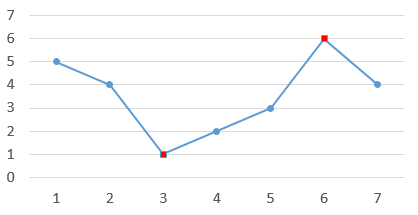
\includegraphics{chapter3/exam201604_1/p1.png}
    \caption{折点示意图}
    \label{fig:201604-1-1}
\end{figure}

给定$n$个整数$a_1,a_2,\cdots,a_n$表示销售量,请计算出这些天总共有多少个折点。

为了减少歧义,我们给定的数据保证:在这$n$天中相邻两天的销售量总是不同的,即$a_{i-1} \neq a_i$。注意,如果两天不相邻,销售量可能相同。

\subsection{输入格式}

输入的第一行包含一个整数$n$。

第二行包含$n$个整数,用空格分隔,分别表示$a_1,a_2,\cdots,a_n$。

\subsection{输出格式}

输出一个整数,表示折点出现的数量。

\subsection{样例输入}

\begin{lstlisting}[numbers=none]
7
5 4 1 2 3 6 4
\end{lstlisting}

\subsection{样例输出}

\begin{lstlisting}[numbers=none]
2
\end{lstlisting}

\subsection{评测用例规模与约定}

所有评测用例满足:$1\leq n\leq1000$,每天的销售量是不超过10000的非负整数。

\subsection{对讲义中代码的点评或纠错}
清晰简单: 代码结构相对简单,易于理解。它有一个主循环,用于逐个读取输入的整数,并在每次迭代中检查条件。\\
\indent
使用了有意义的变量名: 变量名命名得相对清晰,例如,n用于存储整数的数量,pre和cur用于存储前一个和当前的整数,cnt用于计数满足条件的数字对。\\
\indent 
条件判断简单明了: 条件判断语句 (pre < cur \&\& cur > next) || (pre > cur \&\& cur < next) 是简单明了的,容易理解。
\subsection{自己原创的代码的点评与注释}

首先读取整数 n,表示销售量的天数。然后,读取包含 n 个整数的数组,表示每天的销售量。接下来,程序遍历销售量数组,检查每一天是否为折点,并计算折点的数量。最后,输出折点的数量。

\begin{lstlisting}[language=C++]
    #include <iostream>
    using namespace std;
    
    int main() {
        // 读取输入
        int n;
        cin >> n;
    
        // 读取销售量数组
        int sales[n];
        for (int i = 0; i < n; ++i) {
            cin >> sales[i];
        }
    
        // 计算折点数量
        int count = 0;
        for (int i = 1; i < n - 1; ++i) {
            if ((sales[i] > sales[i - 1] && sales[i] > sales[i + 1]) ||
                (sales[i] < sales[i - 1] && sales[i] < sales[i + 1])) {
                count++;
            }
        }
    
        // 输出结果
        cout << count << endl;
    
        return 0;
    }        
\end{lstlisting}
\section{201609-1 最大波动}

\subsection{题目描述}%题目描述请保留在文档内
小明正在利用股票的波动程度来研究股票。小明拿到了一只股票每天收盘时的价格,他想知道,这
只股票连续几天的最大波动值是多少,即在这几天中某天收盘价格与前一天收盘价格之差的绝对值最
大是多少。
\subsection{输入格式}

输入的第一行包含一个整数$n$,表示小明拿到的收盘价格的连续天数。

第二行包含$n$个正整数,依次表示每天的收盘价格。

\subsection{输出格式}

输出一个整数,表示这只股票这$n$天中的最大波动值。

\subsection{样例输入}

\begin{lstlisting}[numbers=none]
6
2 5 5 7 3 5
\end{lstlisting}

\subsection{样例输出}

\begin{lstlisting}[numbers=none]
4
\end{lstlisting}

\subsection{样例解释}

第四天和第五天之间的波动最大,波动值为 |3 − 7| = 4。

\subsection{评测用例规模与约定}

对于所有评测用例,$2\leq n\leq1000$.股票每一天的价格为 1 到 10000 之间的整数。

\subsection{对讲义中代码的点评或纠错}
清晰简单: 代码结构相对简单,易于理解。主要使用了一个for循环来逐个读取输入的整数,并计算差值。

使用了有意义的变量名: 变量名命名得相对清晰,例如,n用于存储整数的数量,max用于存储最大的差值,pre和cur用于存储前一个和当前的整数。

使用标准库函数: 代码使用了abs函数来计算整数的绝对值,这是一个标准库函数,避免了手动编写绝对值计算的逻辑。

\subsection{自己原创的代码的点评与注释}

首先读取股票连续天数n,然后读取每天的收盘价格并存储在vector中。接下来,通过遍历计算每天与前一天的价格差的绝对值,找到最大波动值并输出。

\begin{lstlisting}[language=C++]
    #include <iostream>
    #include <vector>
    #include <cmath>
    using namespace std;
    
    int main() {
        // 读取股票连续天数
        int n;
        cin >> n;
    
        // 存储每天的收盘价格
        vector<int> prices(n);
        for (int i = 0; i < n; ++i) {
            cin >> prices[i];
        }
    
        // 计算最大波动值
        int maxFluctuation = 0;
        for (int i = 1; i < n; ++i) {
            // 计算每天与前一天的价格差的绝对值
            int fluctuation = abs(prices[i] - prices[i - 1]);
            // 更新最大波动值
            maxFluctuation = max(maxFluctuation, fluctuation);
        }
    
        // 输出最大波动值
        cout << maxFluctuation << endl;
        return 0;
    }
    
\end{lstlisting}
\section{201809-1 卖菜}

\subsection{题目描述}%题目描述请保留在文档内
在一条街上有 n 个卖菜的商店,按 1 至 n 的顺序排成一排,这些商店都卖一种蔬菜。

第一天,每个商店都自己定了一个价格。店主们希望自己的菜价和其他商店的一致,第二天,每
一家商店都会根据他自己和相邻商店的价格调整自己的价格。具体的,每家商店都会将第二天的菜价
设置为自己和相邻商店第一天菜价的平均值(用去尾法取整)。

注意,编号为 1 的商店只有一个相邻的商店 2,编号为 n 的商店只有一个相邻的商店 n − 1,其他
编号为 i 的商店有两个相邻的商店 i − 1 和 i + 1。

给定第一天各个商店的菜价,请计算第二天每个商店的菜价。
\subsection{输入格式}

输入的第一行包含一个整数$n$,表示商店的数量。

第二行包含$n$个整数,依次表示每个商店第一天的菜价。

\subsection{输出格式}

输出一行,包含$n$个正整数,依次表示每个商店第二天的菜价。

\subsection{样例输入}

\begin{lstlisting}[numbers=none]
8
4 1 3 1 6 5 17 9
\end{lstlisting}

\subsection{样例输出}

\begin{lstlisting}[numbers=none]
2 2 1 3 4 9 10 13
\end{lstlisting}

\subsection{评测用例规模与约定}

对于所有评测用例,$2\leq n\leq1000$,第一天每个商店的菜价为不超过 10000 的正整数。

\subsection{对讲义中代码的点评或纠错}
清晰简单: 代码结构相对简单,易于理解。它使用了一个循环来计算移动平均值,然后输出结果。

使用了有意义的变量名: 变量名命名得相对清晰,例如,prices数组用于存储原始价格数据,newprices数组用于存储移动平均值。

使用常量: 代码中使用const int MAX = 1000;来定义了一个常量,以表示数组的最大长度,这有助于提高代码的可维护性。

\subsection{自己原创的代码的点评与注释}

首先读取商店数量和第一天的菜价,然后根据每个商店及其相邻商店的菜价,计算出第二天的菜价。最后,输出第二天每个商店的菜价。

\begin{lstlisting}[language=C++]
    #include <iostream>
    #include <vector>
    
    using namespace std;
    
    int main() {
        // 读取商店数量
        int n;
        cin >> n;
    
        // 读取第一天各个商店的菜价
        vector<int> prices(n);
        for (int i = 0; i < n; ++i) {
            cin >> prices[i];
        }
    
        // 计算第二天每个商店的菜价
        vector<int> nextDayPrices(n);
        for (int i = 0; i < n; ++i) {
            // 初始化平均值为当前商店的菜价
            int average = prices[i];
    
            // 如果不是第一个商店,加上左边商店的菜价
            if (i > 0) {
                average += prices[i - 1];
            }
    
            // 如果不是最后一个商店,加上右边商店的菜价
            if (i < n - 1) {
                average += prices[i + 1];
            }
    
            // 计算平均值并更新第二天的菜价
            nextDayPrices[i] = average / ((i > 0) + 1 + (i < n - 1));
        }
    
        // 输出第二天每个商店的菜价
        for (int i = 0; i < n; ++i) {
            cout << nextDayPrices[i] << " ";
        }
    
        return 0;
    }
    
\end{lstlisting}
\section{201903-1 小中大}

\subsection{题目背景}
在数据分析中,最小值最大值以及中位数是常用的统计信息。

\subsection{题目描述}%题目描述请保留在文档内


\subsection{输入格式}

输入的第一行包含一个整数$n$,表示商店的数量。

第二行包含$n$个整数,依次表示每个商店第一天的菜价。

\subsection{输出格式}

输出一行,包含$n$个正整数,依次表示每个商店第二天的菜价。

\subsection{样例输入}

\begin{lstlisting}[numbers=none]
8
4 1 3 1 6 5 17 9
\end{lstlisting}

\subsection{样例输出}

\begin{lstlisting}[numbers=none]
2 2 1 3 4 9 10 13
\end{lstlisting}

\subsection{评测用例规模与约定}

对于所有评测用例,$2\leq n\leq1000$,第一天每个商店的菜价为不超过 10000 的正整数。

\subsection{对讲义中代码的点评或纠错}
逻辑清晰:代码逻辑相对清晰,通过使用标准库函数$std::max\_element$和$std::min\_element$来查找最大值和最小值,以及计算中位数。

使用标准库:代码充分利用了C++标准库中的向量容器和算法函数,提高了代码的可读性和可维护性。

中位数计算方式:在计算中位数的时候,有一处可能会引发问题。具体来说,当中位数是一个整数时,使用$static\_cast<int>(median)$来截断小数部分是合理的。但在中位数是一个浮点数时,使用$fixed$和$setprecision$来格式化输出可能更好。

输入数据未验证:代码没有对输入数据的合法性进行验证,如果输入的数据不符合要求,可能会导致程序运行错误。建议添加输入数据的验证。
\subsection{自己原创的代码的点评与注释}

首先读入整数n和有序的测量数据,然后计算最大值、中位数和最小值,并按照从大到小的顺序输出这三个值。其中,处理中位数的逻辑根据测量数据的个数是奇数还是偶数进行了不同的分支处理。

\begin{lstlisting}[language=C++]
    #include <iostream>
    #include <vector>
    #include <cmath>  // 用于处理四舍五入
    
    using namespace std;
    
    int main() {
        // 读入数据
        int n;
        cin >> n;
        // 读入有序的测量数据
        vector<int> measurements(n);
        for (int i = 0; i < n; ++i) {
            cin >> measurements[i];
        }
        // 计算最大值、中位数和最小值
        int max_value = measurements[n - 1];  // 最大值即为最后一个元素
        int min_value = measurements[0];      // 最小值即为第一个元素
        int median_index = n / 2;             // 中位数的索引
    
        // 若n为奇数,则中位数即为中间的数;若n为偶数,则中位数为中间两个数的平均值
        int median_value = (n % 2 == 1) ? measurements[median_index] :
                                          round((measurements[median_index - 1] + measurements[median_index]) / 2.0);
        // 输出结果,按照从大到小的顺序输出
        cout << max_value << " " << median_value << " " << min_value << endl;
    
        return 0;
    }    
\end{lstlisting}
\section{202203-1 未初始化警告}

\subsection{题目背景}

\subsection{问题描述}

\subsection{输入格式}

\subsection{输出格式}

\subsection{样例 1 输入}

\subsection{样例 1 输出}

\subsection{样例解释}

\subsection{评测用例规模与约定}

\subsection{对讲义中代码的点评或纠错}
 
优点:

简洁明了: 代码结构简单,逻辑清晰,易于理解。主要使用了循环、条件语句和向量等基本结构,使得代码整体较为简洁。

使用标准库: 使用了 C++ 标准库中的 vector 容器,简化了对一系列元素的管理,提高了代码的可读性和可维护性。

良好的变量命名: 使用了有意义的变量名,如 initialized、$uninitialized\_count$ 等,有助于理解代码的含义。

对数组越界进行了处理: 在定义 vector<bool> initialized(n + 1, false) 时,考虑到数组索引从 1 开始,避免了数组越界的问题。

合理使用布尔类型: 使用布尔类型的向量,减小了内存占用,提高了空间效率。

\subsection{自己原创的代码的点评与注释}

数据结构选择: 使用一个布尔型的 vector(initialized)来记录每个变量是否已被初始化,通过下标与变量编号对应。

遍历赋值语句: 使用一个循环遍历每一条赋值语句,检查右值是否已经被初始化。

未初始化右值计数: 对于每一条赋值语句,如果右值是一个变量且未被初始化,就将未初始化右值的计数器加一。

更新左值状态: 每次处理完一条赋值语句后,将左值标记为已被初始化。

输出结果: 最后输出未初始化右值的赋值语句数量。

\begin{lstlisting}[language=C++]
    #include <iostream>
    #include <vector>
    #include <unordered_set>
    
    using namespace std;
    
    int main() {
        // 读入变量数量和赋值语句的条数
        int n, k;
        cin >> n >> k;
    
        // 初始化变量是否已被赋值的集合
        vector<bool> initialized(n + 1, false);
    
        // 初始化未初始化右值计数器
        int uninitializedCount = 0;
    
        // 处理每一条赋值语句
        for (int i = 0; i < k; ++i) {
            int xi, yi;
            cin >> xi >> yi;
    
            // 如果右值是变量,检查是否已被初始化
            if (yi > 0 && !initialized[yi]) {
                // 未被初始化,增加计数器
                uninitializedCount++;
            }
    
            // 将左值标记为已被初始化
            initialized[xi] = true;
        }
    
        // 输出未初始化右值的赋值语句条数
        cout << uninitializedCount << endl;
    
        return 0;
    }    
\end{lstlisting}
\section{201703-1 分蛋糕}

\subsection{题目背景}

\subsection{问题描述}

\subsection{输入格式}

\subsection{输出格式}

\subsection{样例 1 输入}

\subsection{样例 1 输出}

\subsection{样例解释}

\subsection{评测用例规模与约定}

\subsection{对讲义中代码的点评或纠错}
 
优点:

简洁而高效的算法: 代码使用了一次循环,通过累加元素值的方式高效地计算满足条件的分组数量,算法简洁而有效。

使用常量和数组: 使用了常量 maxn 来定义数组的最大长度,提高了代码的可维护性。同时,使用数组 a 存储输入元素,对于序列数据结构的处理更加方便。

避免了全局变量: 除了常量 maxn,所有变量都被限制在 main 函数的局部作用域内,避免了全局变量可能带来的问题。

使用 cur 优雅地跟踪当前累加和: 使用 cur 变量巧妙地跟踪当前累加和,提高了代码的可读性。

合理的输入处理: 通过使用循环读取输入,对于数组的初始化和元素的输入都采用了一致的方式。

清晰的逻辑结构: 代码逻辑清晰,易于理解。通过一个循环遍历数组,累加元素值,判断是否满足条件,并更新计数器,最后输出结果。

\subsection{自己原创的代码的点评与注释}

读入蛋糕的数量n和每个朋友至少要分到的蛋糕重量k。

读入n个蛋糕的重量。

对蛋糕重量数组进行排序。

遍历排序后的蛋糕数组,依次将蛋糕分给朋友,每次分给朋友后检查总重量是否达到k。

输出分到蛋糕的朋友数量。

\begin{lstlisting}[language=C++]
    #include <iostream>
    #include <vector>
    #include <algorithm>
    
    using namespace std;
    
    int main() {
        // 读入 n 和 k
        int n, k;
        cin >> n >> k;
    
        // 读入蛋糕的重量数组
        vector<int> weights(n);
        for (int i = 0; i < n; ++i) {
            cin >> weights[i];
        }
    
        // 对蛋糕重量数组进行排序
        sort(weights.begin(), weights.end());
    
        // 初始化朋友计数器和当前朋友所分蛋糕的总重量
        int friendCount = 0;
        int currentWeight = 0;
    
        // 遍历蛋糕,分给朋友
        for (int i = 0; i < n; ++i) {
            // 当前朋友分到的蛋糕总重量加上当前蛋糕的重量
            currentWeight += weights[i];
            
            // 如果当前蛋糕分给朋友后总重量大于等于 k,表示当前朋友分到蛋糕
            if (currentWeight >= k) {
                // 重置当前朋友分到的蛋糕总重量,为下一个朋友做准备
                currentWeight = 0;
                // 朋友计数器加一
                friendCount++;
            }
        }
    
        // 输出结果
        cout << friendCount << endl;
    
        return 0;
    }    
\end{lstlisting}
\section{201612-1 中间数}

\subsection{题目背景}

\subsection{问题描述}

\subsection{输入格式}

\subsection{输出格式}

\subsection{样例 1 输入}

\subsection{样例 1 输出}

\subsection{样例解释}

\subsection{评测用例规模与约定}

\subsection{对讲义中代码的点评或纠错}
 
优点:

直观的算法: 算法直接遍历数组,对每个元素统计左右两侧较小和较大元素的数量,通过比较判断是否为平衡点。算法直观易懂。

使用 vector 动态数组: 使用了 vector 动态数组,提高了代码的灵活性和可维护性,无需显式指定数组的大小。

清晰的变量命名: 使用了具有描述性的变量名,例如 smaller 和 larger,有助于理解代码逻辑。

合理的条件判断: 在内层循环中使用 continue 跳过了与自身比较的情况,避免了不必要的计数。

\subsection{自己原创的代码的点评与注释}

首先对整数序列进行排序,然后找到排序后的中间位置的元素。接着,通过$count_if$函数分别统计小于和大于中间数的元素个数,最后比较这两个数量。如果相等,则存在中间数,输出中间数的值;否则,输出-1表示不存在中间数。

\begin{lstlisting}[language=C++]
    #include <iostream>
    #include <vector>
    #include <algorithm>
    
    using namespace std;
    
    int main() {
        // 读取输入的整数序列长度
        int n;
        cin >> n;
    
        // 读取整数序列
        vector<int> nums(n);
        for (int i = 0; i < n; ++i) {
            cin >> nums[i];
        }
    
        // 对整数序列进行排序
        sort(nums.begin(), nums.end());
    
        // 判断中间数是否存在
        int middleIndex = n / 2; // 中间数的下标
        int middleValue = nums[middleIndex]; // 中间数的值
        int countLess = count_if(nums.begin(), nums.end(), [&](int x) { return x < middleValue; });
        int countGreater = count_if(nums.begin(), nums.end(), [&](int x) { return x > middleValue; });
    
        // 输出结果
        if (countLess == countGreater) {
            cout << middleValue << endl; // 存在中间数,输出中间数的值
        } else {
            cout << -1 << endl; // 不存在中间数,输出-1
        }
    
        return 0;
    }    
\end{lstlisting}
\section{201812-1 小明上学}

\subsection{题目背景}

小明是汉东省政法大学附属中学的一名学生,他每天都要骑自行车往返于家和学校。为了能尽可能充足地睡眠,他希望能够预计自己上学所需要的时间。他上学需要经过数段道路,相邻两段道路之间设有至多一盏红绿灯。

京州市的红绿灯是这样工作的:每盏红绿灯有红、黄、绿三盏灯和一个能够显示倒计时的显示牌。假设红绿灯被设定为红灯$r$秒,黄灯$y$秒,绿灯$g$秒,那么从$0$时刻起,$[0,r)$秒内亮红灯,车辆不许通过;$[r, r+g)$秒内亮绿灯,车辆允许通过;$[r+g, r+g+y)$秒内亮黄灯,车辆不许通过,然后依次循环。倒计时的显示牌上显示的数字$l(l > 0)$是指距离下一次信号灯变化的秒数。

\subsection{问题描述}

一次上学的路上,小明记录下了经过每段路的时间,和各个红绿灯在小明到达路口时的颜色和倒计时秒数。希望你帮忙计算此次小明上学所用的时间。

\subsection{输入格式}

输入的第一行包含空格分隔的三个正整数$r$、$y$、$g$,表示红绿灯的设置。这三个数均不超过 $10^6$。

输入的第二行包含一个正整数 $n(n\leq 100)$,表示小明总共经过的道路段数和看到的红绿灯数目。

接下来的$n$行,每行包含空格分隔的两个整数$k$、$t$。$k=0$ 表示经过了一段道路,耗时$t$秒,此处$t$不超过 $10^6$;$k=1$、$2$、$3$ 时,分别表示看到了一个红灯、黄灯、绿灯,且倒计时显示牌上显示的数字是$t$,此处$t$分别不会超过$r$、$y$、$g$。
 
\subsection{输出格式}

输出一个数字,表示此次小明上学所用的时间。

\subsection{样例 1 输入}

\begin{lstlisting}[numbers=none]
30 3 30
8
0 10
1 5
0 11
2 2
0 6
0 3
3 10
0 3
\end{lstlisting}

\subsection{样例 1 输出}

\begin{lstlisting}[numbers=none]
70
\end{lstlisting}

\subsection{样例解释}

小明先经过第一段道路,用时 10 秒,然后等待 5 秒的红灯,再经过第二段道路,用时 11 秒,然后等待 2 秒的黄灯和 30 秒的红灯,再经过第三段、第四段道路,分别用时6、3秒,然后通过绿灯,再经过最后一段道路,用时 3 秒。共计 $10 + 5 + 11 + 2 + 30 + 6 + 3 + 3=70$ 秒。

\subsection{评测用例规模与约定}

测试点 1, 2 中不存在任何信号灯。
测试点 3, 4 中所有的信号灯在被观察时均为绿灯。
测试点 5, 6 中所有的信号灯在被观察时均为红灯。
测试点 7, 8 中所有的信号灯在被观察时均为黄灯。
测试点 9, 10 中将出现各种可能的情况。

\subsection{对讲义中代码的点评或纠错}
逻辑清晰:代码采用了简单的if-else语句来处理不同情况,逻辑相对清晰,易于理解。

变量命名:变量的命名相对清晰,例如r、y、g分别代表红灯、黄灯、绿灯的时间,n代表车辆数量等。

没有错误处理:代码假定输入是有效的,但没有进行错误处理。如果输入格式不符合要求,可能会导致程序崩溃或产生不正确的结果。
\subsection{自己原创的代码的点评与注释}

读取红绿灯的设置。

读取道路段数和红绿灯数目。

遍历每一段道路和红绿灯,根据不同的情况计算总时间。

输出总时间。

\begin{lstlisting}[language=C++]
    #include <iostream>
    using namespace std;
    
    int main() {
        // 读取红绿灯设置
        int r, y, g;
        cin >> r >> y >> g;
    
        // 读取道路段数和红绿灯数目
        int n;
        cin >> n;
    
        int totalTime = 0; // 记录总时间
    
        for (int i = 0; i < n; ++i) {
            int k, t; // k表示道路或红绿灯类型,t表示经过道路的时间或倒计时时间
            cin >> k >> t;
    
            if (k == 0) {
                // 经过道路的情况
                totalTime += t;
            } else {
                // 遇到红绿灯的情况
                if (k == 1) {
                    // 红灯,需要等待
                    totalTime += (r - t);
                } else if (k == 2) {
                    // 黄灯,需要等待
                    totalTime += (r + g - t);
                }
                // 绿灯无需等待,直接通过
            }
        }
    
        cout << totalTime << endl;
    
        return 0;
    }
    
\end{lstlisting}
\section{201812-2 小明放学}

\subsection{题目背景}

汉东省政法大学附属中学所在的光明区最近实施了名为“智慧光明”的智慧城市项目。具体到交通领域,通过“智慧光明”终端,可以看到光明区所有红绿灯此时此刻的状态。小明的学校也安装了
“智慧光明”终端,小明想利用这个终端给出的信息,估算自己放学回到家的时间。

\subsection{问题描述}

一次放学的时候,小明已经规划好了自己回家的路线,并且能够预测经过各个路段的时间。同时,小明通过学校里安装的“智慧光明”终端,看到了出发时刻路上经过的所有红绿灯的指示状态。请帮忙计算小明此次回家所需要的时间。

\subsection{输入格式}

输入的第一行包含空格分隔的三个正整数 $r、y、g$,表示红绿灯的设置。这三个数均不超过$10^6$。

输入的第二行包含一个正整数$n$,表示小明总共经过的道路段数和路过的红绿灯数目。

接下来的$n$行,每行包含空格分隔的两个整数$k、t$。$k = 0$ 表示经过了一段道路,将会耗时 $t$ 秒,此处 $t$ 不超过 $10^6$;$k$ = 1、2、3 时,分别表示出发时刻,此处的红绿灯状态是红灯、黄灯、绿灯,且倒计时显示牌上显示的数字是 $t$,此处 t 分别不会超过 $r、y、g$。

\subsection{输出格式}

输出一个数字,表示此次小明放学回家所用的时间。

\subsection{样例 1 输入}

\begin{lstlisting}[numbers=none]
    30 3 30
    8
    0 10
    1 5
    0 11
    2 2
    0 6
    0 3
    3 10
    0 3
\end{lstlisting}

\subsection{样例 1 输出}

\begin{lstlisting}[numbers=none]
46
\end{lstlisting}

\subsection{样例解释}

小明先经过第一段路,用时 10 秒。第一盏红绿灯出发时是红灯,还剩 5 秒;小明到达路口时,这个红绿灯已经变为绿灯,不用等待直接通过。接下来经过第二段路,用时 11 秒。第二盏红绿灯出发时是黄灯,还剩两秒;小明到达路口时,这个红绿灯已经变为红灯,还剩 11 秒。接下来经过第三、第四段路,用时 9 秒。第三盏红绿灯出发时是绿灯,还剩 10 秒;小明到达路口时,这个红绿灯已经变为红灯,还剩两秒。接下来经过最后一段路,用时 3 秒。共计 10 + 11 + 11 + 9 + 2 + 3 = 46 秒。

\subsection{评测用例规模与约定}

有些测试点具有特殊的性质:前 2 个测试点中不存在任何信号灯。测试点的输入数据规模:前6个测试点保证$n ≤ 10^3$;所有测试点保证$n ≤ 10^5$。

\subsection{对讲义中代码的点评或纠错}
 
功能实现简单: 代码实现了模拟红绿灯的功能,逻辑相对清晰,容易理解。

变量命名清晰: 变量命名相对清晰,例如$r、y、g$表示红、黄、绿灯的时间,n表示输入的次数等。

未考虑非法输入的情况: 没有处理可能的非法输入情况,比如负数的时间或无效的灯类型。

\subsection{自己原创的代码的点评与注释}

根据输入的每一段路的类型(道路或红绿灯),累加小明经过的时间。对于红绿灯,根据其状态和倒计时时间,计算小明需要等待的时间。

\begin{lstlisting}[language=C++]
    #include <iostream>

    using namespace std;
    
    int main() {
        // 红绿灯的设置
        int r, y, g;
        cin >> r >> y >> g;
    
        // 小明总共经过的道路段数和路过的红绿灯数目
        int n;
        cin >> n;
    
        // 初始化总时间
        int total_time = 0;
    
        // 遍历每一段路
        for (int i = 0; i < n; ++i) {
            int k, t;
            cin >> k >> t;
    
            if (k == 0) {
                // 如果是道路,直接加上时间
                total_time += t;
            } else {
                // 如果是红绿灯
                if (k == 1) {
                    // 红灯,需要等待剩余时间
                    total_time += t;
                } else if (k == 2) {
                    // 黄灯,需要等待剩余时间,同时加上红灯的时间
                    total_time += t + r;
                } else {
                    // 绿灯,直接通过
                }
            }
        }
    
        cout << total_time << endl;
    
        return 0;
    }    
\end{lstlisting}
\section{202006-1 线性分类器}

\subsection{问题描述}

考虑一个简单的二分类问题——将二维平面上的点分为 A 和 B 两类。
训练数据包含 n 个点,其中第 i 个点 (1 ≤ i ≤ n) 可以表示为一个三元组 (xi
, yi
, typei),即该点的
横坐标、纵坐标和类别。
在二维平面上, 任意一条直线可以表示为 θ0 + θ1x + θ2y = 0 的形式,即由 θ0、θ1 和 θ2 三个参数
确定该直线,且满足 θ1、θ2 不同时为 0 。
基于这 n 个已知类别的点,我们想要在平面上找到一条直线作为一个线性分类器。具体来说,这
条线要把训练数据中的 A、B 两类点完美分隔开来,即一侧只有 A 类点、另一侧只有 B 类点。这样,
对于任意一个的末知类别的点,我们就可以根据它是位于直线的哪一侧来预测它的类别了。

在本题中我们仅需要处理 m 个如下查询:给定一条直线,判断它是否能将训练数据中的 A、B 两
类点完美分开。
\subsection{输入格式}

从标准输入读入数据。
输入共 n + m + 1 行。
第一行包含用空格分隔的两个正整数 n 和 m,分别表示点和查询的个数。
第二行到第 n+ 1 行依次输入 n 个点的信息。第 i+ 1 行 (1 ≤ i ≤ n) 包含用空格分割的三项 xi、yi、
typei,分别代表第 i 个点的横、纵坐标和类别,其中坐标为整数、类别为一个大写英文字母 A 或 B。
第 n + 2 行到第 n + m + 1 行依次输入 m 个查询。第 j + n + 1 行 (1 ≤ j ≤ m) 包含用空格分隔的
三个整数 θ0、θ1 和 θ2,表示第 j 个查询中给定直线的三个参数。

\subsection{输出格式}

输出到标准输出。
输出共 m 行,每行输出一个字符串。
第 j 行 (1 ≤ j ≤ m) 输出的字符串对应第 j 个查询的结果:如果给定直线可以完美分隔 A、B 两
类点,则输出 Yes;否则输出 No。

\subsection{样例输入}

\begin{lstlisting}[numbers=none]
9 3
1 1 A
1 0 A
1 -1 A
2 2 B
2 3 B
0 1 A
3 1 B
1 3 B
2 0 A
0 2 -3
-3 0 2
-3 1 1
\end{lstlisting}

\subsection{样例输出}

\begin{lstlisting}[numbers=none]
    No
    No
    Yes
\end{lstlisting}

\subsection{样例解释}

如图3.2所示,只有第 3 个查询给出的直线能将 A、B 两类点完美分隔。

\subsection{子任务}

有些测试点具有特殊的性质:前 2 个测试点中不存在任何信号灯。测试点的输入数据规模:前6个测试点保证$n ≤ 10^3$;所有测试点保证$n ≤ 10^5$。

\subsection{对讲义中代码的点评或纠错}
 
清晰明了的逻辑: 代码逻辑相对清晰,容易理解。通过输入点的坐标和类型,然后根据给定的直线参数,判断两组点是否被该直线分开。

使用了C++的标准库: 使用了C++的标准库中的vector和pair,这样可以更方便地管理和操作点集合。

变量命名: 变量命名相对明确,有助于理解代码的功能。

合理利用bool类型: 使用布尔类型来表示条件的真假,提高了代码的可读性。

未处理输入异常: 代码没有对输入进行异常处理。如果输入不符合预期,可能导致程序行为不可预测。建议添加一些输入验证机制,确保程序稳健性。

\subsection{自己原创的代码的点评与注释}

首先读取点的信息,然后根据查询的直线参数判断是否能够完美分隔,并输出结果。

\begin{lstlisting}[language=C++]
    #include <iostream>
    #include <vector>
    
    using namespace std;
    
    // 定义点的结构体
    struct Point {
        int x, y;
        char type;
    };
    
    // 判断点在直线的哪一侧
    int classifyPoint(Point p, int theta0, int theta1, int theta2) {
        int result = theta0 + theta1 * p.x + theta2 * p.y;
        if (result > 0) {
            return 1; // 点在直线上方
        } else {
            return -1; // 点在直线下方或在直线上
        }
    }
    
    // 判断是否能完美分隔A、B两类点
    bool canSeparate(vector<Point>& points, int theta0, int theta1, int theta2) {
        for (Point& p : points) {
            int classification = classifyPoint(p, theta0, theta1, theta2);
            if (classification * (p.type == 'A' ? 1 : -1) <= 0) {
                // 若分类结果与实际类别不一致,则不能完美分隔
                return false;
            }
        }
        return true; // 所有点都正确分类,可以完美分隔
    }
    
    int main() {
        int n, m;
        cin >> n >> m;
    
        // 读取点的信息
        vector<Point> points(n);
        for (int i = 0; i < n; ++i) {
            cin >> points[i].x >> points[i].y >> points[i].type;
        }
    
        // 读取查询的直线参数
        for (int j = 0; j < m; ++j) {
            int theta0, theta1, theta2;
            cin >> theta0 >> theta1 >> theta2;
    
            // 判断是否能完美分隔,并输出结果
            if (canSeparate(points, theta0, theta1, theta2)) {
                cout << "Yes" << endl;
            } else {
                cout << "No" << endl;
            }
        }
    
        return 0;
    }    
\end{lstlisting}
\section{201509-2 日期计算}

\subsection{题目背景}

\subsection{问题描述}

\subsection{输入格式}

\subsection{输出格式}

\subsection{样例 1 输入}

\subsection{样例 1 输出}

\subsection{样例解释}

\subsection{评测用例规模与约定}

\subsection{对讲义中代码的点评或纠错}
 
优点:

简洁明了的逻辑: 代码逻辑相对简单,清晰易懂。通过判断是否为闰年,然后根据每个月的天数计算月份和天数。

使用数组存储月份天数: 使用数组$normal$存储每个月的天数,提高了代码的可读性和维护性。

使用布尔类型表示是否为闰年: 使用$leap\_year$布尔变量表示是否为闰年,增加了代码的可读性。

缺点和改进空间:

未处理输入异常: 代码没有对输入进行异常处理。如果输入不符合预期,可能导致程序行为不可预测。建议添加一些输入验证机制,确保程序稳健性。

\subsection{自己原创的代码的点评与注释}

编写一个函数 isLeapYear 判断是否为闰年,根据题目中的条件进行判断。

编写一个函数 calculateDate 根据输入的年份和天数计算月份和日期。

在 main 函数中读取输入的年份和天数,调用 calculateDate 函数计算结果,最后输出月份和日期。

\begin{lstlisting}[language=C++]
    #include <iostream>
    using namespace std;
    // 判断是否为闰年的函数
    bool isLeapYear(int year) {
        return (year % 4 == 0 && year % 100 != 0) || (year % 400 == 0);
    }
    // 计算某年某一天是几月几日的函数
    void calculateDate(int year, int dayOfYear, int &month, int &day) {
        // 定义每个月的天数
        int daysInMonth[] = {0, 31, 28, 31, 30, 31, 30, 31, 31, 30, 31, 30, 31};
    
        // 如果是闰年,2月的天数为29
        if (isLeapYear(year)) {
            daysInMonth[2] = 29;
        }
        // 初始化月份和日期
        month = 1;
        day = 0;
        // 循环减去每个月的天数,直到剩余天数小于等于当前月的天数
        while (dayOfYear > daysInMonth[month]) {
            dayOfYear -= daysInMonth[month];
            month++;
        }
        // 剩余的天数即为日期
        day = dayOfYear;
    }
    int main() {
        // 输入年份和天数
        int year, dayOfYear;
        cin >> year >> dayOfYear;
    
        // 计算月份和日期
        int month, day;
        calculateDate(year, dayOfYear, month, day);
    
        // 输出结果
        cout << month << endl;
        cout << day << endl;
    
        return 0;
    }    
\end{lstlisting}
\section{201503-3 节日}

\subsection{题目背景}

\subsection{问题描述}

\subsection{输入格式}

\subsection{输出格式}

\subsection{样例 1 输入}

\subsection{样例 1 输出}

\subsection{样例解释}

\subsection{评测用例规模与约定}

\subsection{对讲义中代码的点评或纠错}
 
优点:

使用结构体: 使用结构体Date将日期相关的信息封装在一起,提高了代码的可读性和可维护性。

成员函数的封装: isLeap() 和 daysInMonth() 函数封装了与日期相关的逻辑,使代码更加模块化。

明确函数的功能: 函数和成员变量的命名相对清晰,有助于理解代码的功能。

合理利用结构体成员: 使用结构体成员变量表示年、月、日和星期,使代码更直观。

使用 printf 进行格式化输出: 使用 printf 提高了输出格式的灵活性和可读性。

处理日期的逻辑清晰: addOneDay() 函数处理日期的逻辑相对清晰,考虑了月末和年末的进位。

bool isLastDay() 函数的逻辑非常简单,通过逻辑与运算符$\&\&$检查当前日期的月份是否为12(即12月),且日期是否为31日,这种简单直接的实现有助于减少代码的复杂性和错误的可能性。
并且这个函数体现了面向对象编程的封装性。通过将日期相关的逻辑封装在结构体内部,提高了代码的模块化和可维护性。

缺点和改进空间:

输入异常处理: 缺少对输入的合法性检查。应该考虑在读入a、b、c、y1和y2之前添加输入合法性的检查,以确保输入的有效性。

\subsection{自己原创的代码的点评与注释}

getFirstDayOfWeek 函数用于计算某年某月第一天是星期几, calculateDate 函数用于计算某年某月第 b 个星期 c 的日期。在 main 函数中,按照要求输出结果。

\begin{lstlisting}[language=C++]
    #include <iostream>
    #include <iomanip>
    
    using namespace std;
    
    // 判断是否是闰年的函数
    bool isLeapYear(int year) {
        if (year % 400 == 0 || (year % 4 == 0 && year % 100 != 0)) {
            return true;
        }
        return false;
    }
    
    // 计算某年某月第一天是星期几的函数
    int getFirstDayOfWeek(int year, int month) {
        // 已知 1850 年 1 月 1 日是星期二
        int days = 0;
        for (int i = 1850; i < year; ++i) {
            days += isLeapYear(i) ? 366 : 365;
        }
        for (int i = 1; i < month; ++i) {
            switch (i) {
                case 1: case 3: case 5: case 7: case 8: case 10: case 12:
                    days += 31;
                    break;
                case 4: case 6: case 9: case 11:
                    days += 30;
                    break;
                case 2:
                    days += isLeapYear(year) ? 29 : 28;
                    break;
            }
        }
        return (days + 2) % 7;  // 2 corresponds to the first day being Tuesday
    }
    
    // 计算某年某月第 b 个星期 c 的日期的函数
    string calculateDate(int year, int month, int b, int c) {
        int firstDayOfWeek = getFirstDayOfWeek(year, month);
        int targetDay = c - firstDayOfWeek + (b - 1) * 7;
    
        // 如果 targetDay 小于等于零或者大于该月的天数,表示不存在符合条件的日期
        if (targetDay <= 0 || targetDay > 31) {
            return "none";
        }
    
        // 如果 targetDay 大于该月的天数,取最后一天
        int daysInMonth;
        switch (month) {
            case 1: case 3: case 5: case 7: case 8: case 10: case 12:
                daysInMonth = 31;
                break;
            case 4: case 6: case 9: case 11:
                daysInMonth = 30;
                break;
            case 2:
                daysInMonth = isLeapYear(year) ? 29 : 28;
                break;
        }
    
        if (targetDay > daysInMonth) {
            targetDay = daysInMonth;
        }
    
        // 格式化输出日期
        stringstream ss;
        ss << year << "/" << setw(2) << setfill('0') << month << "/" << setw(2) << setfill('0') << targetDay;
        return ss.str();
    }
    
    int main() {
        int a, b, c, y1, y2;
        cin >> a >> b >> c >> y1 >> y2;
    
        for (int year = y1; year <= y2; ++year) {
            string result = calculateDate(year, a, b, c);
            cout << result << endl;
        }
    
        return 0;
    }    
\end{lstlisting}

\chapter{STL入门与vector}
\begin{introduction}[本人完成的题目]
  \item 
  \begin{enumerate}[\Roman*]
      \item 一维 vector
   \begin{enumerate}[\arabic*]
       \item 201712-2 游戏
       \item 202009-2 风险人群筛查
   \end{enumerate}
\item 二维 vector
    \begin{enumerate}[\arabic*]
       \item 201503-1 图像旋转
       \item 201512-2 消除类游戏
       \item 201604-2 俄罗斯方块
       \item 202305-2 矩阵运算
   \end{enumerate}
\item 结构体与 vector
    \begin{enumerate}[\arabic*]
      \item 201403-2 窗口
      \item 201803-2 碰撞的小球
      \item 201912-2 回收站选址
      \item 202009-1 检测点查询
   \end{enumerate}
\item pair 与 vector
  \begin{enumerate}[\arabic*]
    \item 202006-2 稀疏向量
    \item 202206-2 寻宝!大冒险!
  \end{enumerate}
  \end{enumerate}
\end{introduction}
\section{201712-2 游戏}

\subsection{题目背景}

\subsection{问题描述}

\subsection{输入格式}

\subsection{输出格式}

\subsection{样例 1 输入}

\subsection{样例 1 输出}

\subsection{样例解释}

\subsection{评测用例规模与约定}

\subsection{对讲义中代码的点评或纠错}
 
优点:

使用了标准库vector:使用了C++的标准库vector来存储每个人的编号,这是一个合适的选择,可以方便地进行插入和删除操作。

简洁的初始化:利用循环简洁地初始化了children向量,使其包含1到n的编号。

使用了合理的循环结构:使用了两个嵌套循环结构,其中外层循环迭代直到只剩下一个人,内层循环处理报数的逻辑。

缺点和改进空间:

不够高效:使用erase操作来删除vector中的元素,这涉及到移动后续元素,导致时间复杂度较高,特别是当k较大时。可以考虑使用链表等数据结构,以提高删除操作的效率。

未处理输入异常:代码没有对输入进行异常处理,如果输入不符合预期,可能导致程序行为不可预测。建议添加一些输入验证机制,确保程序稳健性。

\subsection{自己原创的代码的点评与注释}

使用一个数组来表示每个小朋友是否被淘汰。在循环中,按照规则报数,淘汰符合条件的小朋友,直到只剩下一个小朋友为止。最后输出获胜小朋友的编号。

\begin{lstlisting}[language=C++]
    #include <iostream>
    using namespace std;
    
    int main() {
        // 读取输入的 n 和 k
        int n, k;
        cin >> n >> k;
    
        // 定义一个数组表示小朋友是否被淘汰,初始都为 false
        bool eliminated[1001] = {false};
    
        // 初始化报数和当前小朋友编号
        int count = 0;
        int current = 1;
    
        // 当还有多于一个小朋友时进行循环
        while (count < n - 1) {
            // 如果当前小朋友没有被淘汰
            if (!eliminated[current]) {
                // 报数加1
                count++;
    
                // 如果报的数是 k 的倍数或者末位数为 k,则淘汰当前小朋友
                if (count % k == 0 || count % 10 == k) {
                    eliminated[current] = true;
                    count--;
                }
            }
    
            // 移动到下一个小朋友
            current = (current % n) + 1;
        }
    
        // 输出最后获胜的小朋友编号
        for (int i = 1; i <= n; i++) {
            if (!eliminated[i]) {
                cout << i << endl;
                break;
            }
        }
    
        return 0;
    }    
\end{lstlisting}
\section{202009-2 风险人群筛查}

\subsection{题目背景}

\subsection{问题描述}

\subsection{输入格式}

\subsection{输出格式}

\subsection{样例 1 输入}

\subsection{样例 1 输出}

\subsection{样例解释}

\subsection{评测用例规模与约定}

\subsection{对讲义中代码的点评或纠错}
 
优点:

合理的数据结构选择: 使用了两个vector<int>来存储通过和滞留的人数,这是合理的选择,可以方便地对结果进行统计。

合理的循环嵌套结构: 使用了两层嵌套循环,外层遍历人,内层遍历时间,对每个人在每个时间点的位置进行判断。这样的结构较为清晰。

逻辑清晰: 通过布尔变量inside来表示人是否在矩形区域内,通过cnt来表示连续在矩形区域内的时间数,逻辑相对清晰。

合理的变量命名: 变量命名相对清晰,有助于理解代码的功能

缺点和改进空间:

未处理输入异常: 代码没有对输入进行异常处理。如果输入不符合预期,可能导致程序行为不可预测。建议添加一些输入验证机制,确保程序稳健性。

\subsection{自己原创的代码的点评与注释}

通过循环读取每个居民的位置记录。

遍历位置记录,判断每个时刻是否位于高危区域内。

统计经过高危区域的人数(有任意一个时刻在高危区域内即可)。

判断是否曾在高危区域逗留,需要连续 k 个或更多时刻在高危区域内。

\begin{lstlisting}[language=C++]
    #include <iostream>
    #include <vector>
    
    using namespace std;
    
    int main() {
        // 读取输入参数
        int n, k, t, xl, yd, xr, yu;
        cin >> n >> k >> t >> xl >> yd >> xr >> yu;
    
        // 记录经过高危区域和逗留的人数
        int passCount = 0, stayCount = 0;
    
        // 遍历每个居民
        for (int i = 0; i < n; ++i) {
            // 读取居民的位置记录
            vector<pair<int, int>> positions;
            for (int j = 0; j < t; ++j) {
                int x, y;
                cin >> x >> y;
                positions.push_back({x, y});
            }
    
            // 记录连续位于高危区域的次数
            int consecutiveCount = 0;
    
            // 遍历位置记录
            for (int j = 0; j < t; ++j) {
                // 判断是否位于高危区域
                if (positions[j].first >= xl && positions[j].first <= xr &&
                    positions[j].second >= yd && positions[j].second <= yu) {
                    // 位于高危区域,连续计数加一
                    consecutiveCount++;
                } else {
                    // 不位于高危区域,重置连续计数
                    consecutiveCount = 0;
                }
    
                // 判断是否满足逗留条件
                if (consecutiveCount >= k) {
                    stayCount++;
                    break; // 已经满足逗留条件,不再判断后续时刻
                }
            }
    
            // 判断是否经过高危区域
            if (consecutiveCount > 0) {
                passCount++;
            }
        }
    
        // 输出结果
        cout << passCount << endl;
        cout << stayCount << endl;
    
        return 0;
    }
\end{lstlisting}
\section{201503-1 图像旋转}

\subsection{题目背景}

\subsection{问题描述}

\subsection{输入格式}

\subsection{输出格式}

\subsection{样例 1 输入}

\subsection{样例 1 输出}

\subsection{样例解释}

\subsection{评测用例规模与约定}

\subsection{对讲义中代码的点评或纠错}
 
优点:

使用了标准库 vector: 代码使用了C++标准库中的 vector 来表示二维矩阵,这是一个合理的选择,方便了矩阵的动态创建和访问。

合理的输入循环: 使用了嵌套循环,逐行逐列读取输入矩阵的元素,使得输入过程比较清晰。

合理的矩阵旋转逻辑: 使用两个嵌套循环,从右向左遍历每一列,再从上到下遍历每一行,输出逆时针旋转后的结果。

缺点和改进空间:

未处理输入异常: 代码没有对输入进行异常处理。如果输入不符合预期,可能导致程序行为不可预测。建议添加一些输入验证机制,确保程序稳健性。

\subsection{自己原创的代码的点评与注释}

首先读取图像矩阵的行数和列数,然后读入图像矩阵。接着,它创建一个新的矩阵rotatedMatrix来存储逆时针旋转90度后的结果。最后,通过两层嵌套循环遍历原始矩阵,将每个元素按照旋转规则放置到新矩阵中。最终,输出旋转后的矩阵。

\begin{lstlisting}[language=C++]
    #include <iostream>
    #include <vector>
    
    using namespace std;
    
    int main() {
        // 读入图像矩阵的行数和列数
        int n, m;
        cin >> n >> m;
    
        // 读入图像矩阵
        vector<vector<int>> matrix(n, vector<int>(m));
        for (int i = 0; i < n; ++i) {
            for (int j = 0; j < m; ++j) {
                cin >> matrix[i][j];
            }
        }
    
        // 逆时针旋转矩阵
        // 注意:旋转后的行数变为原来的列数,列数变为原来的行数
        vector<vector<int>> rotatedMatrix(m, vector<int>(n));
    
        for (int i = 0; i < n; ++i) {
            for (int j = 0; j < m; ++j) {
                // 逆时针旋转 90 度后,原矩阵的第i行第j列元素,变为旋转后矩阵的第j行第(n-1-i)列元素
                rotatedMatrix[j][n - 1 - i] = matrix[i][j];
            }
        }
    
        // 输出旋转后的矩阵
        for (int i = 0; i < m; ++i) {
            for (int j = 0; j < n; ++j) {
                cout << rotatedMatrix[i][j] << " ";
            }
            cout << endl;
        }
    
        return 0;
    }    
\end{lstlisting}
\section{201512-2 消除类游戏}

\subsection{题目背景}

\subsection{问题描述}

\subsection{输入格式}

\subsection{输出格式}

\subsection{样例 1 输入}

\subsection{样例 1 输出}

\subsection{样例解释}

\subsection{评测用例规模与约定}

\subsection{对讲义中代码的点评或纠错}
 
优点:

使用了标准库 vector: 代码使用了C++标准库中的 vector 来表示矩阵和判断矩阵,这是一个合理的选择,方便了矩阵的动态创建和访问。

合理的嵌套循环结构: 使用了两个嵌套循环,遍历整个矩阵,检测并处理连续相同元素的情况。

清晰的判断条件: 通过判断条件 if (j + 2 < m $\&\&$ ...) 和 if (i + 2 < n $\&\&$ ...),清晰地表达了寻找连续相同元素的条件。

输出格式控制: 输出时通过三目运算符控制输出 0 或者原元素值,使得输出格式较为整齐。

缺点和改进空间:

未处理输入异常: 代码没有对输入进行异常处理。如果输入不符合预期,可能导致程序行为不可预测。建议添加一些输入验证机制,确保程序稳健性。

\subsection{自己原创的代码的点评与注释}

遍历每一行和每一列,查找是否存在连续三个或更多相同颜色的棋子,如果存在则将它们标记为0表示消除。最后输出消除后的棋盘。

\begin{lstlisting}[language=C++]
    #include <iostream>
    #include <vector>
    
    using namespace std;
    
    // 定义一个函数,用于在一行或一列中查找并消除连续三个或更多相同颜色的棋子
    void eliminate(vector<vector<int>>& board, int n, int m) {
        // 检查每一行
        for (int i = 0; i < n; ++i) {
            for (int j = 0; j <= m - 3; ++j) {
                if (board[i][j] == board[i][j + 1] && board[i][j + 1] == board[i][j + 2]) {
                    // 将连续三个相同颜色的棋子标记为0,表示消除
                    board[i][j] = board[i][j + 1] = board[i][j + 2] = 0;
                }
            }
        }
    
        // 检查每一列
        for (int j = 0; j < m; ++j) {
            for (int i = 0; i <= n - 3; ++i) {
                if (board[i][j] == board[i + 1][j] && board[i + 1][j] == board[i + 2][j]) {
                    // 将连续三个相同颜色的棋子标记为0,表示消除
                    board[i][j] = board[i + 1][j] = board[i + 2][j] = 0;
                }
            }
        }
    }
    
    int main() {
        // 读取棋盘的行数和列数
        int n, m;
        cin >> n >> m;
    
        // 读取棋盘上每个方格的颜色
        vector<vector<int>> board(n, vector<int>(m));
        for (int i = 0; i < n; ++i) {
            for (int j = 0; j < m; ++j) {
                cin >> board[i][j];
            }
        }
    
        // 调用消除函数
        eliminate(board, n, m);
    
        // 输出消除后的棋盘
        for (int i = 0; i < n; ++i) {
            for (int j = 0; j < m; ++j) {
                cout << board[i][j] << " ";
            }
            cout << endl;
        }
    
        return 0;
    }    
\end{lstlisting}
\section{201604-2 俄罗斯方块}

\subsection{题目背景}

\subsection{问题描述}

\subsection{输入格式}

\subsection{输出格式}

\subsection{样例 1 输入}

\subsection{样例 1 输出}

\subsection{样例解释}

\subsection{评测用例规模与约定}

\subsection{对讲义中代码的点评或纠错}
 
优点:

使用了常量定义: 使用 $const int GRID\_SIZE = 20$; 定义了常量,提高了代码的可读性和可维护性。

使用了 memcpy 进行数组拷贝: 使用了 memcpy 进行数组 grid 到 tmp 的拷贝,这是一种高效的拷贝方式。

函数抽象: 将尝试放置方块的逻辑抽象成了 tryPlaceBlock 函数,提高了代码的可读性和可维护性。

在最下面一行增加一层代码: 在 for 循环中增加了一行代码 grid[15][i] = 1;在方格图 grid 最下面增加一层地板,这样做的目的是简化边界检查逻辑,增加了游戏性。

缺点和改进空间:

全局变量使用: 使用了全局变量 row 和 col,这样的全局变量容易导致命名空间污染,建议将其作为局部变量传递给需要的函数。

未考虑输入异常: 代码没有对输入进行异常处理。如果输入不符合预期,可能导致程序行为不可预测。建议添加一些输入验证机制,确保程序稳健性。

\subsection{自己原创的代码的点评与注释}

接受输入,模拟俄罗斯方块板块下落,并输出最终的方格图。主要思路是从底部找到板块的落脚点,然后将板块复制到方格图中。函数printGrid用于输出方格图,函数dropBlock用于模拟板块下落。

\begin{lstlisting}[language=C++]
    #include <iostream>
    using namespace std;
    
    const int ROWS = 15;
    const int COLS = 10;
    
    // 函数声明
    void printGrid(int grid[ROWS][COLS]);
    void dropBlock(int grid[ROWS][COLS], int block[4][4], int col);
    
    int main() {
        // 读取初始方格图
        int grid[ROWS][COLS];
        for (int i = 0; i < ROWS; ++i) {
            for (int j = 0; j < COLS; ++j) {
                cin >> grid[i][j];
            }
        }
    
        // 读取板块形状
        int block[4][4];
        for (int i = 0; i < 4; ++i) {
            for (int j = 0; j < 4; ++j) {
                cin >> block[i][j];
            }
        }
    
        // 读取板块初始位置
        int col;
        cin >> col;
    
        // 模拟板块下落
        dropBlock(grid, block, col);
    
        // 输出最终方格图
        printGrid(grid);
    
        return 0;
    }
    
    // 输出方格图
    void printGrid(int grid[ROWS][COLS]) {
        for (int i = 0; i < ROWS; ++i) {
            for (int j = 0; j < COLS; ++j) {
                cout << grid[i][j] << " ";
            }
            cout << endl;
        }
    }
    
    // 模拟板块下落
    void dropBlock(int grid[ROWS][COLS], int block[4][4], int col) {
        // 从底部开始找到板块的落脚点
        int row = ROWS - 1;
        while (row >= 0 && block[3][col] == 0) {
            row--;
        }
    
        // 将板块复制到方格图中
        for (int i = 0; i < 4; ++i) {
            for (int j = 0; j < 4; ++j) {
                if (block[i][j] == 1) {
                    grid[row + i][col + j] = 1;
                }
            }
        }
    }    
\end{lstlisting}

\subsection{你推荐的代码}

\href{201604-2 俄罗斯方块}{https://blog.csdn.net/tigerisland45/article/details/54790942}

\subsection{网上的代码}
\begin{lstlisting}[language=C++]
    #include <iostream>
     
    const int ROW = 15;
    const int COL = 10;
    const int N = 4;
     
    int board[ROW+1][COL];
    int block[N][N];
    struct {
        int row, col;
    } coords[N];
     
    using namespace std;
     
    int main()
    {
        int row, col;
     
        // 输入数据
        for(int i=0; i<ROW; i++)
            for(int j=0; j<COL; j++)
                cin >> board[i][j];
        for(int i=0; i<N; i++)
            for(int j=0; j<N; j++)
                cin >> block[i][j];
        cin >> col;
     
        // 底边全放1
        for(int j=0; j<COL; j++)
            board[ROW][j] = 1;
     
        // 提取小方块坐标
        int k = 0;
        for(int i=N-1; i>=0; i--)
            for(int j=0; j<N; j++)
                if(block[i][j] == 1) {
                    coords[k].row = i;
                    coords[k].col = j;
                    k++;
                }
     
        // 模拟小方块落下过程
        row = 1;
        col--;
        bool checkflag;
        for(;;) {
            checkflag = false;
     
            for(int i=0; i<N; i++)
                if(board[row + coords[i].row][col + coords[i].col] == 1) {
                    checkflag = true;
                    break;
                }
     
            if(checkflag)
                break;
     
            row++;
        }
        row--;
     
        // 合并小方块到方格
        for(int i=0; i<N; i++)
            board[row + coords[i].row][col + coords[i].col] = 1;
     
        // 输出结果
        for(int i=0; i<ROW; i++) {
            for(int j=0; j<COL; j++) {
                if(j != 0)
                    cout << " ";
                cout << board[i][j];
            }
            cout << endl;
        }
     
        return 0;
    }
\end{lstlisting}
\section{202305-2 矩阵运算}

\subsection{题目背景}

\subsection{问题描述}

\subsection{输入格式}

\subsection{输出格式}

\subsection{样例 1 输入}

\subsection{样例 1 输出}

\subsection{样例解释}

\subsection{评测用例规模与约定}

\subsection{对讲义中代码的点评或纠错}
 
优点:

使用了合适的数据结构:使用了二维向量(vector of vectors)来表示矩阵,这是一个在C++中灵活且方便的数据结构。

代码结构清晰:通过使用嵌套的循环,代码结构相对清晰,易于理解。

使用了适当的数据类型:在矩阵乘法过程中,使用了long long类型来处理可能的溢出问题,保证了计算结果的准确性。

缺点和改进空间:

未进行错误检查:代码没有对输入数据的合法性进行验证,如果输入的数据不符合要求,可能会导致程序运行错误。建议添加输入数据的验证。

\subsection{自己原创的代码的点评与注释}

通过嵌套的循环读取矩阵 Q、K、V 以及向量 W 的元素。

在计算结果时,利用嵌套循环遍历矩阵元素,按照题目描述的公式进行计算。

输出计算结果。

\begin{lstlisting}[language=C++]
    #include <iostream>
    #include <vector>
    using namespace std;
    int main() {
        // 读取输入数据
        int n, d;
        cin >> n >> d;
    
        // 读取矩阵 Q
        vector<vector<int>> Q(n, vector<int>(d));
        for (int i = 0; i < n; ++i) {
            for (int j = 0; j < d; ++j) {
                cin >> Q[i][j];
            }
        }
    
        // 读取矩阵 K
        vector<vector<int>> K(n, vector<int>(d));
        for (int i = 0; i < n; ++i) {
            for (int j = 0; j < d; ++j) {
                cin >> K[i][j];
            }
        }
    
        // 读取矩阵 V
        vector<vector<int>> V(n, vector<int>(d));
        for (int i = 0; i < n; ++i) {
            for (int j = 0; j < d; ++j) {
                cin >> V[i][j];
            }
        }
    
        // 读取向量 W
        vector<int> W(n);
        for (int i = 0; i < n; ++i) {
            cin >> W[i];
        }
    
        // 计算结果并输出
        for (int i = 0; i < n; ++i) {
            for (int j = 0; j < d; ++j) {
                // 计算 (Q × KT) 中第 i 行的每个元素与 W(i) 相乘的结果,并与 V 相乘
                cout << W[i] * (Q[i][0] * K[i][j] + Q[i][1] * K[i][j] + Q[i][2] * K[i][j]) * V[i][j] << " ";
            }
            cout << endl;
        }
    
        return 0;
    }    
\end{lstlisting}
\section{201403-2 窗口}

\subsection{题目背景}

\subsection{问题描述}

\subsection{输入格式}

\subsection{输出格式}

\subsection{样例 1 输入}

\subsection{样例 1 输出}

\subsection{样例解释}

\subsection{评测用例规模与约定}

\subsection{对讲义中代码的点评或纠错}
 
优点:

使用了结构体:通过定义结构体Window来表示窗口的位置和编号,提高了代码的可读性和结构化程度。

封装了判断点是否在窗口内的函数:使用isInside函数来判断给定的点是否在窗口内,提高了代码的模块化和可维护性。

使用了向量容器:通过使用vector容器来存储窗口信息,方便了对窗口的动态管理,如添加、删除等操作。

基本逻辑清晰:代码逻辑相对清晰,通过嵌套循环实现了窗口选择和置顶的操作。

\subsection{自己原创的代码的点评与注释}

首先定义了一个窗口结构体,包含窗口的坐标信息和顺序编号。然后,它依次读入窗口信息和鼠标点击信息,模拟点击过程并输出结果。在每次点击后,将被点击的窗口移到所有窗口的最顶层。程序使用一个循环遍历窗口来确定最顶层的窗口,并在点击后更新窗口的顺序。

\begin{lstlisting}[language=C++]
    #include <iostream>
    #include <vector>
    
    using namespace std;
    
    // 定义窗口结构体
    struct Window {
        int x1, y1, x2, y2; // 窗口左上角和右下角坐标
        int order;          // 窗口的顺序编号
    };
    
    // 判断点是否在窗口内部
    bool isInside(int x, int y, const Window& window) {
        return x >= window.x1 && x <= window.x2 && y >= window.y1 && y <= window.y2;
    }
    
    int main() {
        int N, M;
        cin >> N >> M;
    
        vector<Window> windows(N);
    
        // 读入窗口信息
        for (int i = 0; i < N; ++i) {
            cin >> windows[i].x1 >> windows[i].y1 >> windows[i].x2 >> windows[i].y2;
            windows[i].order = i + 1; // 窗口编号从1开始
        }
    
        // 模拟鼠标点击
        for (int i = 0; i < M; ++i) {
            int x, y;
            cin >> x >> y;
    
            bool clicked = false;
            // 从顶层到底层遍历窗口,找到最顶层的窗口
            for (int j = N - 1; j >= 0; --j) {
                if (isInside(x, y, windows[j])) {
                    cout << windows[j].order << endl;
                    // 将当前点击的窗口移至顶层
                    Window clickedWindow = windows[j];
                    windows.erase(windows.begin() + j);
                    windows.push_back(clickedWindow);
                    clicked = true;
                    break;
                }
            }
    
            // 如果没有窗口被点击,则输出IGNORED
            if (!clicked) {
                cout << "IGNORED" << endl;
            }
        }
    
        return 0;
    }    
\end{lstlisting}

\subsection{你推荐的代码}

\href{201403-2 窗口}{https://blog.csdn.net/tigerisland45/article/details/54782238}

\subsection{网上的代码}
\begin{lstlisting}[language=C++]
    #include <iostream>
     
    using namespace std;
     
    const int N = 10;
     
    struct {
        int winno;
        int x1, y1, x2, y2;
    } win[N];
     
    struct {
        int x, y;
    } point[N];
     
    int order[N];
     
    int main()
    {
        int n, m;
     
        // 输入数据
        cin >> n >> m;
        for(int i=0; i<n; i++) {
            win[i].winno = i + 1;
            cin >> win[i].x1 >> win[i].y1 >> win[i].x2 >> win[i].y2;
        }
        for(int i=0; i<m; i++)
            cin >> point[i].x >> point[i].y;
     
        // 初始化窗口显示顺序
        for(int i=0; i<n; i++)
            order[i] = n - i - 1;
     
        // 处理(模拟)鼠标点击
        int winno, temp;
        for(int i=0; i<m; i++) {
            winno = -1;     // 被点击的窗口号,-1表示未被点击
     
            // 判断哪个窗口被点击
            for(int j=0; j<n; j++) {
                if(win[order[j]].x1 <= point[i].x && point[i].x <= win[order[j]].x2 &&
                        win[order[j]].y1 <= point[i].y && point[i].y <= win[order[j]].y2) {
                    // 得到窗口号
                    winno = win[order[j]].winno;
     
                    // 将被点击的窗口移到最前端
                    temp = order[j];
                    for(int k=j; k>0; k--)
                        order[k] = order[k-1];
                    order[0] = temp;
     
                    break;
                }
            }
     
            // 输出结果
            if(winno == -1)
                cout << "IGNORED" << endl;
            else
                cout << winno << endl;
        }
     
        return 0;
    }
\end{lstlisting}
\section{201803-2 碰撞的小球}

\subsection{题目背景}

\subsection{问题描述}

\subsection{输入格式}

\subsection{输出格式}

\subsection{样例 1 输入}

\subsection{样例 1 输出}

\subsection{样例解释}

\subsection{评测用例规模与约定}

\subsection{对讲义中代码的点评或纠错}
 
优点:

使用了结构体:通过定义结构体Ball来表示球的属性,提高了代码的可读性和结构化程度。

使用了函数:通过将球的移动和碰撞模拟封装成了两个函数moveBalls和checkCollisions,提高了代码的模块化和可维护性。

采用了向量容器:通过使用vector容器来存储球的信息,方便了对球的动态管理,如添加、删除等操作。

逻辑清晰:代码逻辑相对清晰,模拟了球的移动和碰撞过程,并在每个时间步骤内更新了球的位置。

缺点和改进空间:

没有进行输入数据的合法性验证:代码没有对输入的数据进行验证,如果输入的数据不符合要求,可能会导致程序运行错误。建议添加输入数据的验证。

\subsection{你推荐的代码}

\href{201803-2 碰撞的小球}{https://blog.csdn.net/tigerisland45/article/details/81660041}

\subsection{网上的代码}
\begin{lstlisting}[language=C++]
    #include <iostream>
    #include <algorithm>
     
    using namespace std;
     
    const int N = 100;
    struct Node {
        int id;         // 小球编号
        int pos;        // 位置
        int step;       // 运动方向,1表示向右,-1表示向左
    } b[N];
     
    bool cmp1(Node a, Node b)
    {
        return a.pos < b.pos;
    }
     
    bool cmp2(Node a, Node b)
    {
        return a.id < b.id;
    }
     
     
    int main()
    {
        int n, l, t, id = 0;
     
        cin >> n >> l >> t;
        for(int i = 0; i < n; i++) {
            b[i].id = ++id;
            cin >> b[i].pos;
            // 开始往右走,到达两端则回头
            b[i].step = 1;
            if(b[i].pos == l || b[i].pos == 0)
                b[i].step = -b[i].step;
        }
     
        sort(b, b + n, cmp1);
        for(int i = 0; i < t; i++) {
            // 走一步
            for(int j = 0; j < n; j++) {
                b[j].pos += b[j].step;
                // 到达两端则回头
                if(b[j].pos == l || b[j].pos == 0)
                    b[j].step = -b[j].step;
            }
     
            // 判断是否碰头,碰头则掉头(排序后只需要比较相邻的)
            for(int j = 1; j < n; j++)
                if(b[j].pos == b[j - 1].pos)
                    b[j].step = -b[j].step, b[j - 1].step = -b[j - 1].step;
        }
     
        sort(b, b + n, cmp2);
        for(int i = 0; i < n; i++)
            cout << b[i].pos << " ";
        cout << endl;
     
        return 0;
    }    
\end{lstlisting}
\section{201912-2 回收站选址}

\subsection{题目背景}

\subsection{问题描述}

\subsection{输入格式}

\subsection{输出格式}

\subsection{样例 1 输入}

\subsection{样例 1 输出}

\subsection{样例解释}

\subsection{评测用例规模与约定}

\subsection{对讲义中代码的点评或纠错}
 
优点:

使用了结构体:通过定义结构体Coordinate来表示坐标点的属性,提高了代码的可读性和结构化程度。

封装了函数:通过将垃圾检查和地址计数的逻辑封装成了两个函数hasGarbage和countAddresses,提高了代码的模块化和可维护性。

使用了向量容器:通过使用vector容器来存储垃圾的坐标,方便了对垃圾的动态管理,如添加、删除等操作。

代码逻辑清晰:通过循环遍历垃圾坐标,进行相应的检查和计数,代码逻辑相对清晰,易于理解。

使用了初始化列表:在Coordinate结构体的构造函数中使用了初始化列表,提高了代码的简洁性和效率。

使用了$emplace\_back$:在向garbage向量中添加元素时使用了$emplace\_back$,避免了不必要的拷贝构造,提高了性能。

缺点和改进空间:

没有进行输入数据的合法性验证:代码没有对输入的数据进行验证,如果输入的数据不符合要求,可能会导致程序运行错误。建议添加输入数据的验证。

\subsection{自己原创的代码的点评与注释}

用$unordered\_set$存储垃圾点坐标,以便快速查找。

遍历每个垃圾点,判断其上下左右四个邻居位置是否都存在垃圾。

计算四个对角位置中存在垃圾的个数,作为得分。

根据条件判断是否满足建站条件,满足则更新相应得分的回收站选址个数。

输出最终结果。

\begin{lstlisting}[language=C++]
    #include <iostream>
    #include <vector>
    #include <unordered_set>
    
    using namespace std;
    
    int main() {
        // 读取输入
        int n;
        cin >> n;
    
        // 垃圾点坐标存储在set中,便于查找
        unordered_set<int> garbage_points;
        
        // 读取垃圾点坐标并存储
        for (int i = 0; i < n; ++i) {
            int x, y;
            cin >> x >> y;
            garbage_points.insert(x * 1000000 + y);  // 将二维坐标转为一维,确保唯一性
        }
    
        // 初始化得分为0的回收站选址个数
        vector<int> scores(5, 0);
    
        // 遍历每个垃圾点,判断是否满足建站条件
        for (auto point : garbage_points) {
            int x = point / 1000000;
            int y = point % 1000000;
    
            // 上下左右四个邻居位置
            bool up = garbage_points.count((x, y + 1));
            bool down = garbage_points.count((x, y - 1));
            bool left = garbage_points.count((x - 1, y));
            bool right = garbage_points.count((x + 1, y));
    
            // 在 (x ± 1, y ± 1) 四个对角位置中有几处存在垃圾
            int diagonal_score = 0;
            diagonal_score += garbage_points.count((x - 1, y - 1));
            diagonal_score += garbage_points.count((x - 1, y + 1));
            diagonal_score += garbage_points.count((x + 1, y - 1));
            diagonal_score += garbage_points.count((x + 1, y + 1));
    
            // 判断是否满足建站条件
            if (up && down && left && right) {
                scores[diagonal_score]++;
            }
        }
    
        // 输出结果
        for (int score : scores) {
            cout << score << endl;
        }
    
        return 0;
    }    
\end{lstlisting}

\subsection{你推荐的代码}

\href{201912-2 回收站选址}{https://blog.csdn.net/weixin\_45884316/article/details/103604320}

\subsection{网上的代码}
\begin{lstlisting}[language=C++]
    #include<stdio.h>
    int main()
    {
        long long int a[1000][2];
        int b[1000]={0},c[5]={0};
        int n,i,j;
        scanf("%d",&n);
        for(i=0;i<n;i++)
            scanf("%lld%lld",&a[i][0],&a[i][1]);//数组的值为坐标 
        for(i=0;i<n;i++)
        {
            for(j=i+1;j<n;j++)
            {
                if((a[i][0]==a[j][0]&&a[i][1]==a[j][1]+1)||(a[i][0]==a[j][0]&&a[i][1]==a[j][1]-1)||	(a[i][0]==a[j][0]-1&&a[i][1]==a[j][1])||(a[i][0]==a[j][0]+1&&a[i][1]==a[j][1]))
                {
                    b[i]++;
                    b[j]++;
                }
            }
        }
        for(i=0;i<n;i++)
        {
            int count=0;//对角线上有几个 
            if(b[i]==4)
            {
                for(j=0;j<n;j++)
                {
                    if((a[i][0]==a[j][0]+1&&a[i][1]==a[j][1]+1)||(a[i][0]==a[j][0]+1&&a[i][1]==a[j][1]-1)||
                    (a[i][0]==a[j][0]-1&&a[i][1]==a[j][1]+1)||(a[i][0]==a[j][0]-1&&a[i][1]==a[j][1]-1))
                        count++;
                }
                c[count]++;
            } 
        }
        for(i=0;i<=4;i++)
            printf("%d\n",c[i]);
        return 0;
    }    
\end{lstlisting}
\section{202009-1 检测点查询}

\subsection{题目背景}

\subsection{问题描述}

\subsection{输入格式}

\subsection{输出格式}

\subsection{样例 1 输入}

\subsection{样例 1 输出}

\subsection{样例解释}

\subsection{评测用例规模与约定}

\subsection{对讲义中代码的点评或纠错}
 
优点:

使用了结构体:通过定义结构体 Checkpoint 来表示检查点的属性,提高了代码的可读性和结构化程度。

封装了函数:通过将计算距离、比较和筛选最近检查点的逻辑封装成了函数 distance、compare 和 $nearest\_checkpoints$,提高了代码的模块化和可维护性。

使用了标准库:通过使用 C++ 标准库中的 sort 函数,简化了对检查点的排序操作。

使用了 Lambda 表达式:在 sort 函数的参数中使用了 Lambda 表达式,提高了代码的简洁性,避免了额外的函数定义。

考虑了相等情况下的排序:在 compare 函数中,当两个检查点距离相等时,按照 ID 递增顺序排序,保证了排序的稳定性。

使用了向量容器:通过使用 vector 容器来存储检查点的信息,方便了对检查点的动态管理,如添加、删除等操作。

代码逻辑清晰:通过适当的命名和结构,代码逻辑相对清晰,易于理解。

缺点和改进空间:

没有进行输入数据的合法性验证:代码没有对输入的数据进行验证,如果输入的数据不符合要求,可能会导致程序运行错误。建议添加输入数据的验证。

没有错误处理:程序没有考虑除数为零的情况,当检查点数量为零时,可能导致计算距离的函数 distance 中的除法出现问题。应该在代码中添加相应的错误处理逻辑。

\subsection{自己原创的代码的点评与注释}

定义结构体DetectionPoint表示检测点,包含编号和坐标信息。

编写计算两点之间距离的函数calculateDistance。

编写比较函数compareDistance,用于sort排序时按距离从小到大排序,如果距离相同,则按编号从小到大排序。

在主函数中,读取输入,存储检测点信息,并使用sort函数对检测点进行排序。

输出距离最近的三个检测点的编号。

\begin{lstlisting}[language=C++]
    #include <iostream>
    #include <vector>
    #include <cmath>
    #include <algorithm>
    
    using namespace std;
    
    // 定义检测点结构体,包含编号和坐标信息
    struct DetectionPoint {
        int id;
        int x;
        int y;
    };
    
    // 计算两点之间的距离
    double calculateDistance(int x1, int y1, int x2, int y2) {
        return sqrt(pow(x1 - x2, 2) + pow(y1 - y2, 2));
    }
    
    // 比较函数,用于sort排序时按距离从小到大排序
    bool compareDistance(const DetectionPoint& a, const DetectionPoint& b, int citizenX, int citizenY) {
        double distanceA = calculateDistance(a.x, a.y, citizenX, citizenY);
        double distanceB = calculateDistance(b.x, b.y, citizenX, citizenY);
    
        // 如果距离相同,按编号从小到大排序
        if (distanceA == distanceB) {
            return a.id < b.id;
        }
    
        return distanceA < distanceB;
    }
    
    int main() {
        // 读取输入
        int n, citizenX, citizenY;
        cin >> n >> citizenX >> citizenY;
    
        // 存储检测点信息的数组
        vector<DetectionPoint> detectionPoints(n);
    
        // 读取每个检测点的坐标信息
        for (int i = 0; i < n; ++i) {
            detectionPoints[i].id = i + 1;
            cin >> detectionPoints[i].x >> detectionPoints[i].y;
        }
    
        // 使用sort函数对检测点进行排序,排序规则为距离从小到大
        sort(detectionPoints.begin(), detectionPoints.end(), [citizenX, citizenY](const DetectionPoint& a, const DetectionPoint& b) {
            return compareDistance(a, b, citizenX, citizenY);
        });
    
        // 输出距离最近的三个检测点的编号
        for (int i = 0; i < min(3, n); ++i) {
            cout << detectionPoints[i].id << endl;
        }
    
        return 0;
    }    
\end{lstlisting}
\section{202006-2 稀疏向量}

\subsection{题目背景}

\subsection{问题描述}

\subsection{输入格式}

\subsection{输出格式}

\subsection{样例 1 输入}

\subsection{样例 1 输出}

\subsection{样例解释}

\subsection{评测用例规模与约定}

\subsection{对讲义中代码的点评或纠错}
 
优点:

使用了 pair:通过使用 pair 存储键值对,提高了代码的可读性,使得代码中每个元素都有相关联的键。

使用了 vector 容器:通过使用 vector 存储键值对的集合,方便了对键值对的动态管理,如添加、删除等操作。

使用了 long long:在计算结果时,使用了 long long 类型来防止溢出,保证了计算的准确性。

代码逻辑清晰:通过使用两个指针(i 和 j)来遍历两个向量,并根据键的大小比较来计算乘积之和,代码逻辑相对清晰,易于理解。

采用了合理的循环控制:通过使用 while 循环,避免了写繁琐的 for 循环,提高了代码的简洁性。

\subsection{自己原创的代码的点评与注释}

通过 pair<int, int> 存储稀疏表示的向量,其中 first 表示维度的索引,second 表示在该维度上的非零值。

通过两个指针 i 和 j 分别遍历向量 u 和 v 的稀疏表示,比较当前维度的索引值。

根据比较结果更新内积的值。

输出最终计算得到的内积。

\begin{lstlisting}[language=C++]
    #include <iostream>
    #include <vector>
    
    using namespace std;
    
    int main() {
        // 读取输入数据
        int n, a, b;
        cin >> n >> a >> b;
    
        // 用于存储稀疏表示的向量
        vector<pair<int, int>> u_sparse(a);
        vector<pair<int, int>> v_sparse(b);
    
        // 读取向量 u 的稀疏表示
        for (int i = 0; i < a; ++i) {
            cin >> u_sparse[i].first >> u_sparse[i].second;
        }
    
        // 读取向量 v 的稀疏表示
        for (int i = 0; i < b; ++i) {
            cin >> v_sparse[i].first >> v_sparse[i].second;
        }
    
        // 计算内积
        int result = 0;
        int i = 0, j = 0;
    
        while (i < a && j < b) {
            // 如果两个稀疏向量在当前维度上有非零值
            if (u_sparse[i].first == v_sparse[j].first) {
                result += u_sparse[i].second * v_sparse[j].second;
                ++i;
                ++j;
            } else if (u_sparse[i].first < v_sparse[j].first) {
                // 如果向量 u 在当前维度上有非零值而向量 v 没有
                ++i;
            } else {
                // 如果向量 v 在当前维度上有非零值而向量 u 没有
                ++j;
            }
        }
    
        // 输出结果
        cout << result << endl;
    
        return 0;
    }    
\end{lstlisting}
\section{202206-2 寻宝!大冒险!}

\subsection{题目背景}

\subsection{问题描述}

\subsection{输入格式}

\subsection{输出格式}

\subsection{样例 1 输入}

\subsection{样例 1 输出}

\subsection{样例解释}

\subsection{评测用例规模与约定}

\subsection{对讲义中代码的点评或纠错}
 
优点:

使用了结构体和 pair:通过定义结构体 pair<int, int> 来表示树木的坐标,提高了代码的可读性和结构化程度。

使用了向量容器:通过使用 vector 容器来存储树木的坐标和藏宝图的信息,方便了对树木和藏宝图的动态管理,如添加、删除等操作。

使用了 find 算法:在检查树木的坐标是否存在于树木数组中时,使用了 find 算法,提高了代码的简洁性和可读性。

使用了静态转换:通过使用 $static\_cast$ 对布尔值进行静态类型转换,使得代码更加明确。

代码逻辑清晰:通过嵌套循环逐一检查树木的坐标是否与藏宝图相符,代码逻辑相对清晰,易于理解。

使用了初始化列表:在声明 $treasure\_map$ 时使用了初始化列表,提高了代码的简洁性和效率。

缺点和改进空间:

缺少输入验证:代码没有对输入的数据进行验证,特别是在输入向量大小和元素的情况下。如果输入的数据不符合要求,可能会导致程序运行错误。建议添加输入数据的验证。

\subsection{自己原创的代码的点评与注释}

读取输入数据,包括树的坐标、绿化图和藏宝图的大小。

使用二维向量存储树的坐标和藏宝图。

遍历绿化图上可能的左下角坐标,判断是否存在与藏宝图对应的坐标。

统计满足条件的坐标数量并输出结果。

\begin{lstlisting}[language=C++]
    #include <iostream>
    #include <vector>
    
    using namespace std;
    
    int main() {
        // 读入输入数据
        int n, L, S;
        cin >> n >> L >> S;
    
        // 用于记录树的坐标
        vector<pair<int, int>> treeCoordinates;
    
        // 读入树的坐标
        for (int i = 0; i < n; ++i) {
            int x, y;
            cin >> x >> y;
            treeCoordinates.push_back({x, y});
        }
    
        // 用于记录藏宝图
        vector<vector<int>> treasureMap(S + 1, vector<int>(S + 1));
    
        // 读入藏宝图
        for (int i = S; i >= 0; --i) {
            for (int j = 0; j <= S; ++j) {
                cin >> treasureMap[i][j];
            }
        }
    
        // 统计满足条件的坐标数量
        int count = 0;
    
        // 遍历绿化图上可能的左下角坐标
        for (int x = 0; x <= L - S; ++x) {
            for (int y = 0; y <= L - S; ++y) {
                // 判断是否满足条件
                bool valid = true;
                for (int i = 0; i <= S; ++i) {
                    for (int j = 0; j <= S; ++j) {
                        // 判断绿化图上的坐标是否与藏宝图对应
                        if (treasureMap[i][j] == 1 && treasureMap[i][j] != treeCoordinates[x + i].second) {
                            valid = false;
                            break;
                        }
                    }
                    if (!valid) {
                        break;
                    }
                }
    
                // 如果满足条件,则计数加一
                if (valid) {
                    ++count;
                }
            }
        }
    
        // 输出结果
        cout << count << endl;
    
        return 0;
    }    
\end{lstlisting}

\subsection{你推荐的代码}

\href{202206-2 寻宝!大冒险!}{https://blog.csdn.net/qq\_51800570/article/details/126673741}

\subsection{网上的代码}
\begin{lstlisting}[language=C++]
    #include <iostream>
    #include <cstring>
    #include <algorithm>
    #include <vector>
    
    using namespace std;
    typedef pair <int,int> PII;
    
    vector <PII> v;
    int m[60][60];
    int n, L, S;
    
    bool check(int x, int y)
    {
        //cout << endl;
        for (int i = S; i >= 0; i --)
        {
            for (int j = 0; j <= S; j ++)
            {
                int cx = S - i; //行的逆序,可以选择在存储的地方就改变,也可以在操作时计算原本的下标
                int cy = j;
                //cout << m[i][j] << " " << cx + x << " " << cy + y << endl;
    
                if (x + cx < 0 || x + cx > L || y + cy > L || y + cy < 0) return false; //如果小地图超出大地图的范围,停止
                bool flag = false;
                for (auto t : v)
                {
                    if (x + cx == t.first && y + cy == t.second)
                    {
                        flag = true;
                        break;
                    }
                }
                //cout << m[i][j] << " " << flag << " " << cx + x << " " << cy + y << endl;
                if ((m[i][j] && !flag) || (!m[i][j] && flag)) return false;
            }
        }
        //cout << 1;
        return true;
    }
    
    int main()
    {
        cin >> n >> L >> S;
        memset(m, 0, sizeof(m));
    
        for (int i = 0; i < n; i ++)
        {
            int x, y;
            cin >> x >> y;
            v.push_back({x, y});
            //cout << x << " " << y << endl;
        }
    
        for (int i = 0; i <= S; i ++)
        {
            for (int j = 0; j <= S; j ++)
            {
                cin >> m[i][j]; 
                //最先输入的是 B[S][0]⋯B[S][S] 一行,B[0][0]⋯B[0][S] 一行最后输入
                //不是正宗的数学坐标系啊,只是行的逆序罢了,这个地方卡了我一天,也是挺无语的
            }
        }
    
        int res = 0;
        for (int i = 0; i < n; i ++)
        {
            if (check(v[i].first, v[i].second))
            {
                res ++;
                //cout << v[i].first << " " << v[i].second << endl;
            }
        }
        cout << res;
        return 0;
    }    
\end{lstlisting}

\chapter{STL}
\begin{introduction}[本人完成的题目]
  \item 
  \begin{enumerate}[\Roman*]
      \item list
   \begin{enumerate}[\arabic*]
       \item 201703-2 学生排队
   \end{enumerate}
\item stack 适配器
\item 单调栈适配器
\item $priority\_queue$适配器
    \begin{enumerate}[\arabic*]
       \item 201709-2 公共钥匙盒
   \end{enumerate}
\item map关联
    \begin{enumerate}[\arabic*]
      \item 201312-1 出现次数最多的数
   \end{enumerate}
\item multimap 关联
    \begin{enumerate}[\arabic*]
      \item 201503-2 数字排序
    \end{enumerate}
\item $unordered\_set$无序关联式容器
  \begin{enumerate}[\arabic*]
    \item 201403-1 相反数
  \end{enumerate}
\item $unordered\_map$无序关联式容器
  \begin{enumerate}[\arabic*]
    \item 201412-1 门禁系统
  \end{enumerate}
  \end{enumerate}
\end{introduction}
\section{201703-2 学生排队}

\subsection{题目背景}

\subsection{问题描述}

\subsection{输入格式}

\subsection{输出格式}

\subsection{样例 1 输入}

\subsection{样例 1 输出}

\subsection{样例解释}

\subsection{评测用例规模与约定}

\subsection{对讲义中代码的点评或纠错}
 
优点:

使用了链表容器:通过使用 std::list 链表容器,实现了高效的插入和移动操作,避免了数组的元素移动所带来的开销。

使用了算法库:通过使用 <algorithm> 头文件中的 find 函数,实现了在链表中查找元素的操作,提高了代码的简洁性和可读性。

使用了自动类型推导:在遍历链表元素时使用了 auto 关键字,提高了代码的简洁性。

使用了迭代器:通过使用迭代器对链表进行操作,提高了代码的可读性,并允许在链表中执行高效的插入和移动。

使用了逆向迭代器:在进行负数索引时,使用了 advance 函数和逆向迭代器,实现了从链表末尾开始查找的效果。

代码逻辑清晰:通过使用 std::list 提供的 splice 函数,代码逻辑相对清晰,易于理解。

\subsection{自己原创的代码的点评与注释}

用一个vector保存学生的学号队列,初始化为1到n。

对于每次调整,根据指令进行相应的操作。

向后移动:找到学号为p的学生位置,将其移出队列,然后插入到指定位置。

向前移动:找到学号为p的学生位置,将其移出队列,然后插入到指定位置。

输出最终的学号队列。

\begin{lstlisting}[language=C++]
    #include <iostream>
    #include <vector>
    using namespace std;
    int main() {
        int n, m;
        cin >> n; // 输入学生数量
        cin >> m; // 输入调整次数
    
        vector<int> students; // 保存学生的学号队列
    
        // 初始化学号队列
        for (int i = 1; i <= n; ++i) {
            students.push_back(i);
        }
    
        // 处理每次调整
        for (int i = 0; i < m; ++i) {
            int p, q;
            cin >> p >> q;
    
            // 向后移动
            if (q > 0) {
                vector<int>::iterator it = find(students.begin(), students.end(), p); // 找到学号为p的学生的位置
                int index = distance(students.begin(), it); // 获取位置索引
                students.erase(it); // 将学生移出队列
                students.insert(students.begin() + min(index + q, n), p); // 插入到指定位置
            }
            // 向前移动
            else if (q < 0) {
                vector<int>::iterator it = find(students.begin(), students.end(), p); // 找到学号为p的学生的位置
                int index = distance(students.begin(), it); // 获取位置索引
                students.erase(it); // 将学生移出队列
                students.insert(students.begin() + max(index + q, 0), p); // 插入到指定位置
            }
        }
    
        // 输出最终队列
        for (int i = 0; i < n; ++i) {
            cout << students[i] << " ";
        }
    
        return 0;
    }    
\end{lstlisting}
\section{201709-2 公共钥匙盒}

\subsection{题目背景}

\subsection{问题描述}

\subsection{输入格式}

\subsection{输出格式}

\subsection{样例 1 输入}

\subsection{样例 1 输出}

\subsection{样例解释}

\subsection{评测用例规模与约定}

\subsection{对讲义中代码的点评或纠错}
 
优点:

使用了结构体:通过定义结构体 Event 来表示事件,包含时间、类型和事件id,提高了代码的可读性和结构化程度。

使用了优先队列:通过使用$ priority\_queue $来存储事件,按照时间和事件类型进行排序,实现了按时间顺序处理事件的功能,提高了代码的简洁性和效率。

使用了算法库:通过使用 <algorithm> 头文件中的 find 函数,实现了在向量中查找元素的操作,提高了代码的简洁性和可读性。

使用了结构体的比较函数:通过在结构体中重载 < 运算符,实现了对事件的自定义排序,确保按照时间、类型和id的顺序进行排序。

代码逻辑清晰:通过优先队列的方式,按照事件发生的时间顺序依次处理,代码逻辑相对清晰,易于理解。

考虑了钥匙的状态:在处理事件时,根据事件的类型,更新了钥匙盒的状态,使得钥匙的状态符合事件的影响。

\subsection{自己原创的代码的点评与注释}

使用结构体Teacher存储老师的信息,包括钥匙编号、开始上课时间和上课时长。

创建一个时间线数组,记录每个时刻每个挂钩上的钥匙编号。正数表示老师取钥匙,负数表示老师还钥匙。

模拟老师取还钥匙的过程,根据时间线更新每个挂钩上的钥匙编号。

输出最终钥匙盒里的钥匙顺序。

\begin{lstlisting}[language=C++]
    #include <iostream>
    #include <vector>
    #include <algorithm>
    
    using namespace std;
    
    // 定义老师的结构体,包含钥匙编号、开始上课时间和上课时长
    struct Teacher {
        int keyNumber;
        int startTime;
        int duration;
    };
    
    int main() {
        // 读取输入数据
        int N, K;
        cin >> N >> K;
    
        // 创建老师数组,用于存储老师的信息
        vector<Teacher> teachers(K);
    
        // 读取每位老师的信息
        for (int i = 0; i < K; ++i) {
            cin >> teachers[i].keyNumber >> teachers[i].startTime >> teachers[i].duration;
        }
    
        // 创建时间线数组,用于记录每个时刻每个挂钩上的钥匙编号
        vector<vector<int>> timeline(2 * K + 1, vector<int>(N + 1, 0));
    
        // 处理每位老师的信息
        for (int i = 0; i < K; ++i) {
            int key = teachers[i].keyNumber;  // 获取钥匙编号
            int start = teachers[i].startTime;  // 获取开始上课时间
            int end = start + teachers[i].duration;  // 计算结束上课时间
    
            // 在时间线上标记老师取钥匙和还钥匙的时刻
            timeline[start][key] = i + 1;  // 正数表示取钥匙
            timeline[end][key] = -(i + 1);  // 负数表示还钥匙
        }
    
        // 创建一个数组用于记录每个挂钩上的当前钥匙编号
        vector<int> keyOrder(N + 1);
    
        // 遍历时间线,模拟老师取还钥匙的过程
        for (int i = 1; i <= 2 * K; ++i) {
            for (int j = 1; j <= N; ++j) {
                int action = timeline[i][j];
                if (action > 0) {
                    // 老师取钥匙
                    keyOrder.push_back(j);
                } else if (action < 0) {
                    // 老师还钥匙
                    keyOrder.erase(remove(keyOrder.begin(), keyOrder.end(), -action), keyOrder.end());
                }
            }
        }
    
        // 输出最终钥匙盒里的钥匙顺序
        for (int i = 0; i < N; ++i) {
            cout << keyOrder[i] << " ";
        }
    
        return 0;
    }    
\end{lstlisting}

\subsection{你推荐的代码}

\href{201709-2 公共钥匙盒}{https://blog.csdn.net/weixin\_44572229/article/details/122595406}

\subsection{网上的代码}
\begin{lstlisting}[language=C++]
    #include<iostream>
    #include<algorithm>
    using namespace std;
    const int N=1000;
    struct Node{
        int no;//钥匙编号
        int t;//时间
        int type;//状态 0借  1还
        bool operator<(const Node &a)const 
        {  //按时间从小到大排序 ,如果时间相同,再按照钥匙编号由小到大排序 
            return (t==a.t)?(no<a.no):(t<a.t);
         } 
    }a[2*N];
    int main()
    {
        int n,k,w,s,c,m=0,i,j;
        int ans[N+1];//ans模拟钥匙盒,ans[i]=0表示此位置为空 
        cin>>n>>k;
        for(i=1;i<=n;i++)
          ans[i]=i;//初始化 
        while(k--){
            cin>>w>>s>>c;
            a[m].no=w;
            a[m].t=s;
            a[m++].type=0;//借
            a[m].no=w;
            a[m].t=s+c;
            a[m++].type=1;//还 
        }
        sort(a,a+m);
        for(i=0;i<m;i=j){//i=j是为了保证 i=下个一时间 
            for(j=i;j<m&&a[j].t==a[i].t;j++);
    //先处理同一时间还钥匙 ,编号小的优先还 ,由于时间相同,钥匙编号由小到大排序 故顺序处理即可 
            for(int t=i;t<j;t++)
              if(a[t].type==1){
                  int pos;
                  for(pos=1;pos<=n&&ans[pos];pos++);
                  ans[pos]=a[t].no;
              } 
            // 处理同一时间借钥匙 
            for(int t=i;t<j;t++)
                if(a[t].type==0){
                    int no=a[t].no;
                    int pos;
                    for(pos=1;pos<=n;pos++)//找到要借的钥匙的位置,并标记为借走 
                      if(ans[pos]==no){
                          ans[pos]=0;
                          break;
                      }
                }
        }
        for(i=1;i<=n;i++)
          cout<<ans[i]<<" ";
        cout<<endl;
        return 0; 
    }
\end{lstlisting}
\section{201312-1 出现次数最多的数}

\subsection{题目背景}

\subsection{问题描述}

\subsection{输入格式}

\subsection{输出格式}

\subsection{样例 1 输入}

\subsection{样例 1 输出}

\subsection{样例解释}

\subsection{评测用例规模与约定}

\subsection{对讲义中代码的点评或纠错}
 
优点:

简洁的逻辑结构: 代码逻辑相对简单,易于理解。主要通过 map 统计每个整数的出现次数,然后遍历 map 找到出现次数最多的整数。

使用 STL 容器: 使用了 C++ 标准模板库(STL)中的 map 容器,能够方便地对整数及其出现次数进行管理和排序。

使用迭代器遍历容器: 使用了迭代器 countMap.begin(),能够更方便地遍历 map 容器中的元素。

考虑了相等次数的情况: 在找到出现次数最多的整数时,通过比较键值对的值和键来决定更新结果,考虑了出现次数相等的情况,选择键较小的整数。

合理的注释: 通过简单的注释,对代码中关键步骤和数据结构进行了说明,有助于代码的理解。

使用 auto 关键字: 使用了 auto 关键字,简化了代码,减少了冗余的类型声明。

清晰的变量命名: 变量命名相对清晰,例如 countMap 表示整数出现次数的映射,resultNum 表示结果整数,maxCount 表示最大出现次数。

错误处理: 对于键不存在的情况,map 会自动创建并初始化值为 0,避免了因为键不存在而导致的错误。

\subsection{自己原创的代码的点评与注释}

通过使用$unordered\_map$,我们可以有效地记录每个数字的出现次数。

遍历输入的数字,更新映射中对应数字的出现次数。

在遍历映射时,找到出现次数最多的数字。如果有多个数字出现次数相同,则选择最小的那个。

输出最终结果。

\begin{lstlisting}[language=C++]
    #include <iostream>
    #include <unordered_map>
    #include <climits>
    
    using namespace std;
    
    int main() {
        // 读取输入的 n
        int n;
        cin >> n;
    
        // 创建一个无序映射,用于记录每个数字的出现次数
        unordered_map<int, int> frequencyMap;
    
        // 读取 n 个数字,并在映射中更新它们的出现次数
        for (int i = 0; i < n; ++i) {
            int num;
            cin >> num;
            frequencyMap[num]++;
        }
    
        // 初始化最小的出现次数为最大整数
        int minFrequency = INT_MAX;
    
        // 初始化出现次数最多的数字为0
        int mostFrequentNumber = 0;
    
        // 遍历映射,找出出现次数最多的数字(如果有多个,选择最小的)
        for (const auto& entry : frequencyMap) {
            if (entry.second > minFrequency || (entry.second == minFrequency && entry.first > mostFrequentNumber)) {
                continue; // 如果当前数字的出现次数不大于当前最小出现次数,则跳过
            }
    
            // 更新最小出现次数和出现次数最多的数字
            minFrequency = entry.second;
            mostFrequentNumber = entry.first;
        }
    
        // 输出结果
        cout << mostFrequentNumber << endl;
    
        return 0;
    }    
\end{lstlisting}
\section{201503-2 数字排序}

\subsection{题目背景}

\subsection{问题描述}

\subsection{输入格式}

\subsection{输出格式}

\subsection{样例 1 输入}

\subsection{样例 1 输出}

\subsection{样例解释}

\subsection{评测用例规模与约定}

\subsection{对讲义中代码的点评或纠错}
 
优点:

简洁的逻辑结构: 代码逻辑相对简单,易于理解。主要通过 map 统计每个整数的出现次数,然后使用 multimap 进行排序,最后遍历输出。

使用 STL 容器: 使用了 C++ 标准模板库(STL)中的 map 和 multimap 容器,能够方便地对整数及其出现次数进行管理、排序和输出。

使用 auto 关键字: 使用了 auto 关键字,简化了代码,减少了冗余的类型声明。

清晰的变量命名: 变量命名相对清晰,例如 $count\_map$ 表示整数出现次数的映射,$reversed\_count\_multimap$ 表示按次数降序排列的多重映射。

使用迭代器遍历容器: 使用了迭代器进行容器的遍历,提高了代码的可读性。

正确处理相同次数的整数: 使用 multimap 存储相同次数的整数,保证了在输出时能够按照整数升序排列。

使用 greater 比较器: 在实例化 multimap 时使用了 greater 比较器,确保了次数降序排列。

\subsection{自己原创的代码的点评与注释}

定义一个结构体 NumberCount 来存储整数及其出现的次数。结构体中包含整数 number 和次数 count。

使用 $unordered\_map$ 来统计每个整数出现的次数,其中键是整数值,值是对应的出现次数。

遍历输入的整数序列,更新 countMap 中每个整数的出现次数。

将 countMap 中的统计结果复制到一个 vector 中,每个元素是一个 NumberCount 结构体。

定义 NumberCount 结构体的比较函数,用于排序。排序规则是按出现次数递减排序,如果次数相同,则按整数值递增排序。

使用 std::sort 函数对 numbers 向量进行排序。

输出排序后的结果,即每个整数及其出现次数。

\begin{lstlisting}[language=C++]

    #include <iostream>
    #include <vector>
    #include <unordered_map>
    #include <algorithm>
    
    using namespace std;
    
    struct NumberCount {
        int number;
        int count;
    
        // 构造函数
        NumberCount(int num, int cnt) : number(num), count(cnt) {}
    
        // 用于排序的比较函数
        bool operator<(const NumberCount& other) const {
            // 按出现次数递减排序,如果次数相同,则按数值递增排序
            if (count != other.count) {
                return count > other.count;
            }
            return number < other.number;
        }
    };
    
    int main() {
        int n;
        cin >> n;
    
        unordered_map<int, int> countMap; // 用于统计每个整数出现的次数
        vector<NumberCount> numbers;      // 存储NumberCount结构体,便于排序
    
        for (int i = 0; i < n; ++i) {
            int num;
            cin >> num;
            countMap[num]++;
        }
    
        // 将统计结果存入NumberCount结构体中
        for (const auto& pair : countMap) {
            numbers.emplace_back(pair.first, pair.second);
        }
    
        // 对NumberCount结构体进行排序
        sort(numbers.begin(), numbers.end());
    
        // 输出结果
        for (const auto& numCount : numbers) {
            cout << numCount.number << " " << numCount.count << endl;
        }
    
        return 0;
    }    

\end{lstlisting}
\section{201403-1 相反数}

\subsection{题目背景}

\subsection{问题描述}

\subsection{输入格式}

\subsection{输出格式}

\subsection{样例 1 输入}

\subsection{样例 1 输出}

\subsection{样例解释}

\subsection{评测用例规模与约定}

\subsection{对讲义中代码的点评或纠错}
 
优点:

简洁高效: 代码逻辑相对简单,使用哈希集合 $unordered\_set$ 来实现对相反数的查找。这种方法能够在平均情况下实现 O(1) 的查找效率,从而提高了算法的效率。

使用了哈希集合: 利用哈希集合存储已经遍历过的数字,能够在常数时间内判断是否存在相反数,这在处理大规模数据时效率较高。

用 $unordered\_set$ 避免了排序: 使用哈希集合存储数字,不需要事先对数组进行排序,降低了时间复杂度。

避免了二重循环: 使用哈希集合的方式避免了传统的二重循环查找相反数,减少了算法的时间复杂度。

简单的计数方式: 使用一个变量 count 来计数相反数对的数量,逻辑清晰。

\subsection{自己原创的代码的点评与注释}

使用$unordered\_set$来存储整数,这样可以快速查找一个整数的相反数是否存在。遍历整数数组时,对于每个整数,只需查找其相反数是否在$unordered\_set$中,如果存在,则说明找到了一对相反数。最后,输出计数器的一半,因为每对相反数都被计数了两次。

\begin{lstlisting}[language=C++]

    #include <iostream>
    #include <unordered_set>
    #include <vector>
    
    using namespace std;
    
    int main() {
        int N;
        cin >> N;
        unordered_set<int> numbers;
        vector<int> input(N);
        for (int i = 0; i < N; ++i) {
            cin >> input[i];
            numbers.insert(input[i]);
        }
        int count = 0;
        for (int i = 0; i < N; ++i) {
            if (numbers.count(-input[i]) > 0) {
                count++;
            }
        }
        cout << count / 2 << endl;                // Each pair is counted twice (a and -a)
        return 0;
    }
\end{lstlisting}
\section{201412-1 门禁系统}

\subsection{题目背景}

\subsection{问题描述}

\subsection{输入格式}

\subsection{输出格式}

\subsection{样例 1 输入}

\subsection{样例 1 输出}

\subsection{样例解释}

\subsection{评测用例规模与约定}

\subsection{对讲义中代码的点评或纠错}
 
优点:

简洁明了: 代码逻辑相对简单,主要通过 $unordered\_map$ 实现了对读者编号出现次数的统计。整体结构清晰,易于理解。

使用了标准库容器: 使用了 C++ 标准库中的 $unordered\_map$ 容器,提供了高效的键值对存储和检索功能,不需要手动实现哈希表。

实时更新读者编号出现次数: 在遍历每一条记录时,实时更新对应读者编号在 $unordered\_map$ 中的次数,避免了额外的循环。

适用于大规模数据: 由于使用了哈希表,该算法在平均情况下具有 O(1) 的插入和检索效率,适用于处理大规模数据。

\subsection{自己原创的代码的点评与注释}

使用$unordered\_map$记录每位读者最后一次出现的位置。

对于每条记录,如果读者已经出现过,计算当前次数并更新记录,否则记录为1。

输出结果。

\begin{lstlisting}[language=C++]
    #include <iostream>
    #include <unordered_map>
    #include <vector>
    
    using namespace std;
    
    int main() {
        // 读取记录条数
        int n;
        cin >> n;
    
        // 用unordered_map记录每位读者最后一次出现的位置
        unordered_map<int, int> lastOccurrence;
    
        // 存储每条记录中的读者编号是第几次出现
        vector<int> occurrenceCount;
    
        // 处理每条记录
        for (int i = 0; i < n; ++i) {
            int reader;
            cin >> reader;
    
            // 如果读者已经出现过,更新记录为当前次数
            if (lastOccurrence.find(reader) != lastOccurrence.end()) {
                occurrenceCount.push_back(i - lastOccurrence[reader] + 1);
            } else {
                // 如果是第一次出现,记录为1
                occurrenceCount.push_back(1);
            }
    
            // 更新读者最后一次出现的位置
            lastOccurrence[reader] = i;
        }
    
        // 输出结果
        for (int i = 0; i < n; ++i) {
            cout << occurrenceCount[i];
            if (i < n - 1) {
                cout << " ";
            }
        }
    
        return 0;
    }    
\end{lstlisting}

\chapter{字符串}
\begin{introduction}[本人完成的题目]
  \item 
  \begin{enumerate}[\Roman*]
      \item 字符串函数基础
   \begin{enumerate}[\arabic*]
       \item 201909-3 字符画(复杂模拟)
   \end{enumerate}
\item stl
    \begin{enumerate}[\arabic*]
       \item 201812-3 CIDR合并(vector struct分割)
   \end{enumerate}
\item map 关联式容器
\item $unordered\_map $无序关联式容器
    \begin{enumerate}[\arabic*]
      \item 202305-1 重复局面
      \item 202206-3 角色授权
   \end{enumerate}
\item 分割
\item 复杂模拟
  \begin{enumerate}[\arabic*]
    \item 202012-3 带配额的文件系统(str vec struct)
  \end{enumerate}
  \end{enumerate}
\end{introduction}
\section{201909-3 字符画(复杂模拟)}

\subsection{题目背景}

\subsection{问题描述}

\subsection{输入格式}

\subsection{输出格式}

\subsection{样例 1 输入}

\subsection{样例 1 输出}

\subsection{样例解释}

\subsection{评测用例规模与约定}

\subsection{对讲义中代码的点评或纠错}
 
优点:

模块化设计: 代码采用函数模块化设计,使得不同功能的代码块独立存在,提高了代码的可读性和可维护性。

采用结构体: 使用结构体 ColorRGB 封装了RGB颜色信息,提高了代码的结构性,便于维护和拓展。

使用常量定义: 使用常量 $MAX\_WIDTH$ 和 $MAX\_HEIGHT$ 定义了图像的最大宽度和高度,提高了代码的可读性和可维护性。

合理的注释: 代码中使用了注释,解释了一些关键的步骤和函数的作用,增强了代码的可读性。

灵活的颜色处理: 通过函数 outputBlockColor 实现了对颜色的灵活处理,支持颜色的切换和输出。

使用了标准库函数: 使用了标准库函数,如 cout 和 cin 进行输入输出,提高了代码的易用性。

\subsection{你推荐的代码}

\href{201909-3 字符画}{https://blog.csdn.net/best335/article/details/101296359}

\subsection{网上的代码}
\begin{lstlisting}[language=C++]
    #include<iostream>
    #include<cstring>
    #include<iomanip>
    #include<vector>
    using namespace std;
    unsigned char C[1080][1920][3];//C[n][m][Pixel:RGB] 表示原图片在第n行m列的像素颜色 
    inline unsigned char getPixel(const char&a,const char&b){//将16进制像素数转换为10进制的char 
        return char((isalpha(a)?(10+a-'a'):(a-'0'))*16+(isalpha(b)?(10+b-'a'):(b-'0')));
    }
    inline void outChar(const unsigned char&ch){//输出题意格式化的字符 
        cout<<"\\x"<<hex<<uppercase<<setw(2)<<int(ch);
    }
    inline void outStr(const string& str){//输出题意格式化的字符串 
        for(const char&c:str)outChar(c);
    }
    inline void outPixel(int i){//输出题意格式化的像素 
        vector<int> v;
        if(i==0)v.push_back(0);
        while(i>0) v.push_back(i%10),i/=10;//首先将数按位数分割 例:255 分割为 2、5、5三个数 
        for(i=v.size()-1;i>-1;--i) outChar(char('0'+v[i]));//输出每一位 
    }
    #include<fstream> 
    int main(){
        int m,n,p,q,_B;// W H 
        ifstream cin("C:\\Users\\Isidore\\Desktop\\out.txt");
        cin>>m>>n>>p>>q,_B=p*q,cout.fill('0');
        string s;
        for(int i=0;i<n;++i){
            for(int j=0;j<m;++j){
                cin>>s;
                switch(s.size()){//将s统一格式化为 #abcdef 
                    case 2://#a -> #aaaaaa 
                        s=s+string(5,s[1]);
                        break;
                    case 4://#abc -> #aabbcc
                        s="#"+string(2,s[1])+string(2,s[2])+string(2,s[3]);
                        break;
                }
                for(int k=0;k<3;++k) C[i][j][k]=getPixel(tolower(s[k+k+1]),tolower(s[k+k+2]));
            }
        }
        int R=0,G=0,B=0,r=0,g=0,b=0;
        for(int i=0;i<n;i+=q){//共n/q个字符块行 
            for(int j=0;j<m;j+=p){//每字符块行共m/p段 
                R=0,G=0,B=0;//以下处理属于i行j段的字符块
                for(int k=i,nk=k+q;k<nk;++k)
                    for(int l=j,nl=j+p;l<nl;++l)
                        R+=C[k][l][0],G+=C[k][l][1],B+=C[k][l][2];
                R/=_B,G/=_B,B/=_B;//求平均值 
                if(!(R==r&&G==g&&B==b)){//如果与该行上一段的颜色不同 
                    if(R==0&&G==0&&B==0)//如果与默认值相同 
                        outStr(string(1,char(27))+"[0m");
                    else//其他颜色处理 
                        outStr(string(1,char(27))+"[48;2;"),outPixel(R),outChar(';'),outPixel(G),outChar(';'),outPixel(B),outChar('m');
                    r=R,g=G,b=B;//记录上次的颜色 
                }
                outChar(' ');//输出 (n*m)/(p*q) 个空格 
            }
            if(R!=0||G!=0||B!=0) outStr(string(1,char(27))+"[0m");//行尾判断是否需要重置颜色 
            r=g=b=0;//重置默认颜色 
            outChar('\n');//输出n/q个回车 
        }
        return 0;
    }    
\end{lstlisting}
\section{201812-3 CIDR合并(vector struct分割)}

\subsection{题目背景}

\subsection{问题描述}

\subsection{输入格式}

\subsection{输出格式}

\subsection{样例 1 输入}

\subsection{样例 1 输出}

\subsection{样例解释}

\subsection{评测用例规模与约定}

\subsection{对讲义中代码的点评或纠错}
 
优点:

模块化设计: 代码通过结构体、函数和排序等模块化设计,使得不同功能的代码块独立存在,提高了代码的可读性和可维护性。

使用结构体: 结构体 Node 封装了IP地址和前缀长度,重载了小于操作符,有助于按照指定规则进行排序。

使用标准库: 代码使用了C++标准库提供的数据结构和算法,如 vector 和 sort,提高了代码的可靠性和性能。

合理的注释: 代码中包含了一些注释,解释了关键步骤和函数的作用,提高了代码的可读性。

输入处理: 通过 split 函数对IP地址进行切割,提取出需要的信息,并通过 add 函数将其添加到节点列表中,提高了代码的灵活性。

合并算法: merge 函数实现了合并算法,有效地将CIDR前缀合并,减少了冗余。

\subsection{你推荐的代码}

\href{201812-3 CIDR合并}{https://blog.csdn.net/wingrez/article/details/86601755}

\subsection{网上的代码}
\begin{lstlisting}[language=C++]
    #include<stdio.h>
    #include<stdlib.h>
    #include<string.h>
    #include<algorithm> 
    #define MAXN 1000005
    using namespace std;
    typedef unsigned int UI;
    
    struct IP{
        UI a[5];
        UI val;
    };
    
    int n;
    IP ip[MAXN];
    
    bool cmp(const IP &ip1, const IP &ip2){
        for(int i=0;i<5;i++){
            if(ip1.a[i]!=ip2.a[i]) return ip1.a[i]<ip2.a[i];
        }
        return false;
    }
    
    //将字符串转换为点分十进制形式 
    void deal_str(int no, char *str){
        int pn=0,xn=0;//点的数量,斜杠的数量 
        for(int i=0;i<strlen(str);i++){
            if(str[i]=='.') pn++;
            else if(str[i]=='/') xn++; 
        }
        
        //初始化
        for(int i=0;i<5;i++){
            ip[no].a[i]=0;
        }
        
        //处理字符串 
        int cnt=0;
        char *p1=str, *p2;
        char tmp[5];
        for(int i=0;i<pn;i++){
            p2=strchr(p1,'.');
            strncpy(tmp,p1,p2-p1);
            tmp[p2-p1]=0;
            ip[no].a[cnt++]=atoi(tmp);
            p1=p2+1;
        }
        
        if(xn>0){
            p2=strchr(p1,'/');
            strncpy(tmp,p1,p2-p1);
            tmp[p2-p1]=0;
            ip[no].a[cnt++]=atoi(tmp);
            p1=p2+1;
            strcpy(tmp,p1);
            ip[no].a[4]=atoi(tmp); 
        }
        else{
            strcpy(tmp,p1);
            ip[no].a[cnt++]=atoi(tmp);
            ip[no].a[4]=cnt*8; 
        }
    }
    
    void countVal(int no){ //计算十进制值 
        ip[no].val=0;
        for(int i=0;i<4;i++){
            ip[no].val+=ip[no].a[i]<<8*(3-i);
        }
    }
    
    void range(IP &ip,UI &l, UI &r){ //计算IP前缀能表示的数值范围 
        l=ip.val>>(32-ip.a[4])<<(32-ip.a[4]);
        r=ip.val|((1ull<<(32-ip.a[4]))-1);
    }
    
    void union1(){ //从小到大合并 
        int p=0;
        UI la,ra,lb,rb;
        for(int i=1;i<n;i++){
            range(ip[p],la,ra);
            range(ip[i],lb,rb);
            if(!(la<=lb && rb<=ra)) ip[++p]=ip[i];
        }
        n=p+1; 
    }
    
    bool judge_union(IP &ip1, IP &ip2, IP &res){ //判断同级能否合并 
        if(ip1.a[4]!=ip2.a[4]) return false;
        res=ip1; res.a[4]-=1;
        if(res.a[4]<0) return false;
        UI la,ra,lb,rb,laa,raa;
        range(ip1,la,ra);
        range(ip2,lb,rb);
        range(res,laa,raa);
        if(la==laa && rb==raa && lb<=ra+1) return true;
        return false;
    }
    
    void union2(){
        int p=0;
        IP res;
        for(int i=1;i<n;i++){
            if(judge_union(ip[p],ip[i],res)){
                ip[p]=res;
                while(p>0 && judge_union(ip[p-1], ip[p], res)) ip[--p]=res;
            }
            else ip[++p]=ip[i];
        }
        n=p+1;
    }
    
    int main(){
        char str[25];
        scanf("%d",&n);
        for(int i=0;i<n;i++){
            scanf("%s",str);
            deal_str(i,str);
            countVal(i);
    //		printf("%u.%u.%u.%u/%u\n",ip[i].a[0],ip[i].a[1],ip[i].a[2],ip[i].a[3],ip[i].a[4]);
    //		printf("%u\n",ip[i].val);
        }
        sort(ip,ip+n,cmp);
        union1();
        union2();
        for(int i=0;i<n;i++){
            printf("%u.%u.%u.%u/%u\n",ip[i].a[0],ip[i].a[1],ip[i].a[2],ip[i].a[3],ip[i].a[4]);
        } 
        return 0;
    }    
\end{lstlisting}
\section{202305-1 重复局面}

\subsection{题目背景}

\subsection{问题描述}

\subsection{输入格式}

\subsection{输出格式}

\subsection{样例 1 输入}

\subsection{样例 1 输出}

\subsection{样例解释}

\subsection{评测用例规模与约定}

\subsection{对讲义中代码的点评或纠错}
 
优点:

简洁明了: 代码结构清晰,逻辑简单,容易理解。主要通过$unordered\_map$来记录棋盘局面及其出现的次数。

使用STL容器: 使用了C++标准库提供的$unordered\_map$和vector容器,提高了代码的可读性和易用性。

遵循命名规范: 变量和函数命名符合常见的命名规范,提高了代码的可读性。

输入处理: 通过循环读取每个步骤的局面描述,实现了对不同步骤的处理。

\subsection{自己原创的代码的点评与注释}

使用二维数组positions存储每步棋后的局面。

使用$unordered\_map$统计每个局面出现的次数,其中键为局面的字符串表示,值为出现的次数。

遍历每步棋后的局面,更新局面出现次数并输出。

\begin{lstlisting}[language=C++]
    #include <iostream>
    #include <vector>
    #include <unordered_map>
    
    using namespace std;
    
    int main() {
        int n;
        cin >> n;
    
        vector<vector<string>> positions(n);  // 存储每步棋后的局面
        unordered_map<string, int> positionCount;  // 存储每个局面出现的次数
    
        // 读取每步棋后的局面
        for (int i = 0; i < n; ++i) {
            for (int j = 0; j < 8; ++j) {
                string row;
                cin >> row;
                positions[i].push_back(row);
            }
        }
    
        // 统计每个局面出现的次数
        for (int i = 0; i < n; ++i) {
            string currentPos;
            for (int j = 0; j < 8; ++j) {
                currentPos += positions[i][j];
            }
            positionCount[currentPos]++;
            cout << positionCount[currentPos] << endl;  // 输出当前局面是第几次出现
        }
    
        return 0;
    }    
\end{lstlisting}
\section{202206-3 角色授权}

\subsection{题目背景}

\subsection{问题描述}

\subsection{输入格式}

\subsection{输出格式}

\subsection{样例 1 输入}

\subsection{样例 1 输出}

\subsection{样例解释}

\subsection{评测用例规模与约定}

\subsection{对讲义中代码的点评或纠错}
 
优点:

清晰的结构: 代码模块化,使用了结构体 Role 来存储角色的相关信息,提高了代码的可读性和维护性。

合理使用数据结构: 使用了$unordered\_map$和vector等数据结构,以高效地存储和检索角色及其关联信息。

函数封装: 使用函数将角色信息的读取、关联信息的读取和查询处理分离,提高了代码的模块化程度。

逻辑清晰: 查询处理的逻辑清晰,首先检查个人关联的角色,然后再检查用户组关联的角色,提高了代码的可读性。

使用STL算法: 使用了STL算法中的 find 函数来查找角色操作的可执行性,提高了代码的简洁性。

输入处理: 在读取角色信息和关联信息时,使用了循环和适当的数据结构,处理了多组输入的情况。

\subsection{你推荐的代码}

\href{202206-3 角色授权}{https://blog.csdn.net/qq\_51800570/article/details/126876449}

\subsection{网上的代码}
\begin{lstlisting}[language=C++]
    #include <iostream>
    #include <cstring>
    #include <vector>
    #include <map>
    
    using namespace std;
    
    const int N = 510;
    
    map<string, vector <string> > rolecon; //记录该用户与哪些角色相匹配
    map<string, int> rid; //记录角色所对应的结构体下标
    
    struct role
    {
        string name;
        map <string, int> opset;
        map <string, int> rskind;
        map <string, int> rsname;
    }R[N];
    
    bool check (string rolename, string opname, string rskd, string rsne)
    {
        bool flag = true;
        int id = rid[rolename];
    
        if ((R[id].opset.count("*") == 0) && (R[id].opset.count(opname) == 0)) return false;
        if ((R[id].rskind.count("*") == 0) && (R[id].rskind.count(rskd) == 0)) return false;
        if ((R[id].rsname.size() != 0) && (R[id].rsname.count(rsne) == 0)) return false;
        return true;
    }
    
    int main()
    {
        ios::sync_with_stdio(false);
        int n, m, q;
        cin >> n >> m >> q;
    
        //保存角色内容
        for (int i = 0; i < n; i ++)
        {
            string name;
            cin >> name;
            R[i].name = name;
            rid[name] = i;
    
            int opnum;
            cin >> opnum;
            for (int j = 0; j < opnum; j ++)
            {
                string t;
                cin >> t;
                R[i].opset[t] = 1;
            }
    
            int rk;
            cin >> rk;
            for (int j = 0; j < rk; j ++)
            {
                string t;
                cin >> t;
                R[i].rskind[t] = 1;
            }
    
            int rn;
            cin >> rn;
            for (int j = 0; j < rn; j ++)
            {
                string t;
                cin >> t;
                R[i].rsname[t] = 1;
            }
        }
    
        //存储用户或组分别拥有哪些角色
        for (int i = 0; i < m; i ++)
        {
            string rname;
            cin >> rname;
    
            int rcnt;
            cin >> rcnt;
            for (int j = 0; j < rcnt; j ++)
            {
                string kind, name;
                cin >> kind >> name;
    
                rolecon[name].push_back(rname);
            }
        }
    
        while (q --)
        {
            string pname;
            cin >> pname;
    
            int zulen;
            cin >> zulen;
            vector <string> yongzu;
            for (int i = 0; i < zulen; i ++)
            {
                string t;
                cin >> t;
                yongzu.push_back(t);
            }
            string opname, sk, sn;
            cin >> opname >> sk >> sn;
    
            bool flag = false;
    
            for (int i = 0; i < rolecon[pname].size(); i ++)
            {
                if (check(rolecon[pname][i], opname, sk, sn))
                    {
                        flag = true;
                        break;
                    }
            }
            if (flag)
            {
                cout << 1 << endl;
                continue;
            }
    
            for (int i = 0; i < yongzu.size(); i ++)
            {
                string zname = yongzu[i];
                for (int j = 0; j < rolecon[zname].size(); j ++)
                {
                    if (check(rolecon[zname][j], opname, sk, sn))
                    {
                        flag = true;
                        break;
                    }
                }
                if (flag) break;
            }
            if (flag) cout << 1 << endl;
            else cout << 0 << endl;
        }
    
        return 0;
    }    
\end{lstlisting}
\section{202012-3 带配额的文件系统}

\subsection{题目背景}

\subsection{问题描述}

\subsection{输入格式}

\subsection{输出格式}

\subsection{样例 1 输入}

\subsection{样例 1 输出}

\subsection{样例解释}

\subsection{评测用例规模与约定}

\subsection{对讲义中代码的点评或纠错}
 
优点:

使用了面向对象的设计:通过定义结构体 node 表示文件系统中的节点,包含名称、孩子节点、父节点、文件配额等信息,使用面向对象的思想,提高了代码的可维护性和可扩展性。

使用了动态内存分配:通过使用 new 运算符创建节点,灵活地管理内存,避免了静态内存分配的限制,使得程序更加灵活。

使用了函数和模块化设计:通过将不同功能划分为不同的函数(opec、oper、opeq)和结构体成员函数,实现了代码的模块化设计,提高了代码的可读性和可维护性。

考虑了文件系统的多种操作:程序支持创建、删除文件和目录,以及查询文件和目录的配额信息,覆盖了文件系统的基本操作。

使用了 switch 语句:通过使用 switch 语句处理不同的操作类型,提高了代码的清晰度和可读性。

考虑了根节点的特殊情况:程序在处理根节点时进行了特殊处理,保证了对根节点的操作正确性。

考虑了目录的后代文件配额:在操作普通文件时,考虑了目录及其所有祖先结点的后代文件配额是否满足的问题,保证了数据的一致性。

使用了合适的数据结构:通过使用 vector 存储文件路径,使得路径操作更加灵活。

\subsection{你推荐的代码}

\href{202012-3 带配额的文件系统}{https://blog.csdn.net/qq\_43381135/article/details/112953778}

\subsection{网上的代码}
\begin{lstlisting}[language=C++]
    #include<iostream>
    #include<cstdio>
    #include<map>
    #include<vector>
    #include<cstring>
    #pragma warning (disable:4996)
    using namespace std;
    int num = 0;
    struct node {
        int father; //父节点
        map<string, int>child; //孩子节点
        int type; //1:文件   2:目录
        long long ld, lr;
        long long size;
        long long ld_r, lr_r;
    }Node[4000010];
    vector<pair<int, string> >reback;
    void Reback()
    {
        int i;
        for (i = 0; i < reback.size(); i++)
        {
            int a = reback[i].first;
            string b = reback[i].second;
            Node[a].child.erase(Node[a].child.find(b));
        }
    }
    string executeC()
    {
        int i, j;
        string filepath;
        long long filesize;
        cin >> filepath >> filesize;     //输入普通文件路径以及普通文件大小
        int last = -1;
        for (i = filepath.length() - 1; i >= 0; i--)
        {
            if (filepath[i] == '/')
            {
                last = i;       //找到最后一个/的位置,后面就是文件,前面就是目录
                break;
            }
        }
        int current = 1;
        int id = 0;
        reback.clear();
        int oldnum = num; 
        //前面的目录操作
        while (current < last)
        {
            string t = "";
            while (current < last && filepath[current] != '/')  //读入每一个目录文件的名字
            {
                t = t + filepath[current];
                current++;
            }
            current++;
            if (Node[id].child.find(t) == Node[id].child.end()) //没有这个目录,那就创建一个咯
            {
                num++;
                Node[id].child[t] = num;
                Node[num].father = id;
                Node[num].type = 2;
                Node[num].ld = LLONG_MAX / 3;
                Node[num].lr = LLONG_MAX / 3;
                reback.push_back(make_pair(id, t));
                id = num;
            }
            else                 //存在这个目录文件
            {
                int childid = Node[id].child[t];
                if (Node[childid].type == 1)   //如果这个是文件,则直接输出'N'
                {
                    num = oldnum;
                    Reback();
                    return "N";
                }
                id = childid;
            }
        }
    
        //最后一个的文件操作
        string t = "";
        for (i = last + 1; i < filepath.length(); i++)
        {
            t = t + filepath[i];
        }
        if (Node[id].child.find(t) != Node[id].child.end()) //存在这个文件
        {
            int childid = Node[id].child[t];
            if (Node[childid].type == 2)   //如果这个是目录,直接输出'N'
            {
                num = oldnum;
                Reback();
                return "N";
            }
        }
        //判断新的改变是否满足配额要求
        long long changesize = 0;
        if (Node[id].child.find(t) == Node[id].child.end()) changesize = filesize;
        else changesize = -Node[Node[id].child[t]].size + filesize;
        if (Node[id].ld_r + changesize > Node[id].ld)
        {
            num = oldnum;
            Reback();
            return "N";
        }
        int now = id;
        while (now != -1)
        {
            if (Node[now].lr_r + changesize > Node[now].lr)
            {
                id = oldnum;
                Reback();
                return "N";
            }
            now = Node[now].father;
        }
        //如果满足配额要求,则执行创建普通文件操作以及修改变化的参数
        if (Node[id].child.find(t) == Node[id].child.end())
        {
            num++;
            Node[num].type = 1;
            Node[num].father = id;
            Node[num].size = filesize;
            Node[id].child[t] = num;
        }
        else Node[Node[id].child[t]].size = filesize;
        Node[id].ld_r = Node[id].ld_r + changesize;
        now = id;
        while (now != -1)
        {
            Node[now].lr_r = Node[now].lr_r + changesize;
            now = Node[now].father;
        }
        return "Y";
    }
    string executeR()
    {
        int i;
        string filepath;
        cin >> filepath;          //输入文件路径
        int current = 1;
        int id = 0;
        int last = -1;
        for (i = filepath.length() - 1; i >= 0; i--)
        {
            if (filepath[i] == '/')
            {
                last = i;
                break;
            }
        }
        while (current < last)
        {
            string t = "";
            while (current < last && filepath[current] != '/')
            {
                t = t + filepath[current];
                current++;
            }
            current++;
            if (Node[id].child.find(t) == Node[id].child.end())  //没有这个目录,直接按照删除成功处理
            {
                return "Y";
            }
            else      //存在这个目录,继续扫描下去
            {
                int childid = Node[id].child[t];
                if (Node[childid].type == 1) return "Y";
                id = childid;
            }
        }
        string t = "";
        for (i = last + 1; i < filepath.length(); i++)   //提取最后想要删除的文件名
            t = t + filepath[i];
        if (Node[id].child.find(t) == Node[id].child.end())
            return "Y";
        long long delsize = 0;
        int delNode = Node[id].child[t];     //删除文件的大小
        if (Node[delNode].type == 1)
        {
            Node[id].ld_r = Node[id].ld_r - Node[delNode].size;
            delsize = Node[delNode].size;
            Node[id].child.erase(Node[id].child.find(t));
        }
        else if (Node[delNode].type == 2)
        {
            delsize = Node[delNode].lr_r;
            Node[id].child.erase(Node[id].child.find(t));
        }
        int now = id;
        while (now != -1)
        {
            Node[now].lr_r = Node[now].lr_r - delsize;
            now = Node[now].father;
        }
        return  "Y";
    }
    string executeQ()
    {
        int i;
        string filepath;
        cin >> filepath;
        long long ld, lr;
        cin >> ld >> lr;
        if (ld == 0) ld = LLONG_MAX / 3;
        if (lr == 0) lr = LLONG_MAX / 3;
        int id = 0;
        int last = -1;
        int current = 1;
        for (i = filepath.length() - 1; i >= 0; i--)
        {
            if (filepath[i] == '/')
            {
                last = i;
                break;
            }
        }
        while (current < last)
        {
            string t = "";
            while (current < last && filepath[current] != '/')
            {
                t = t + filepath[current];
                current++;
            }
            current++;
            if (Node[id].child.find(t) == Node[id].child.end())
                return "N";
            else
            {
                int childid = Node[id].child[t];
                if (Node[childid].type == 1) return "N";
                id = childid;
            }
        }
        string t = "";
        for (i = last + 1; i < filepath.length(); i++) t = t + filepath[i];
        int Qnode = 0;
        if (t == "") Qnode = 0;
        else
        {
            if (Node[id].child.find(t) == Node[id].child.end()) return "N";
            else Qnode = Node[id].child[t];
        }
        if (Node[Qnode].type == 1) return "N";
        if (ld < Node[Qnode].ld_r || lr < Node[Qnode].lr_r) return "N";
        Node[Qnode].ld = ld;
        Node[Qnode].lr = lr;
        return "Y";
    }
    int main()
    {
        freopen("in.in", "r", stdin);
        freopen("out.out", "w", stdout);
        int i, j;
        Node[0].type = 2;
        Node[0].ld = LLONG_MAX / 3;
        Node[0].lr = LLONG_MAX / 3;
        Node[0].father = -1;
        int op_num;
        cin >> op_num;   // 输入操作数
        for (i = 1; i <= op_num; i++)
        {
            char op;
            cin >> op;        //输入操作类型
            if (op == 'C')
            {
                cout << executeC() << endl;       //执行创建普通文件操作
            }
            else if (op == 'R')
            {
                cout << executeR() << endl;       //执行移除文件操作
            }
            else if (op == 'Q')
            {
                cout << executeQ() << endl;       //执行设置配额值操作
            }
        }
        return 0;
    }
    
\end{lstlisting}

\end{document}